\documentclass{article}
\usepackage[utf8]{inputenc}
\usepackage{amsmath, amssymb, amsthm}
\usepackage{graphicx, float}
\usepackage{eurosym}
\usepackage{hyperref}
\usepackage{setspace}
\graphicspath{{../images/}}


\doublespacing

\title{
    Exploring the Ability of a Linear Regression Model in Predicting Housing Prices\\[0.7em]
    \large Mathematics: Analysis and Approaches HL \\
    Internal Assessment
}
\author{Nikita Manushin}
\date{June 2026}



\begin{document}

\maketitle


\section{Introduction}

\subsection{Personal Connection}

When I started learning math, in the very first grade, I have always wondered how connected,
the numbers and the real world are. In the past few years Neural Networks became so powerful
they could communicate like humans, all of that using tons of numbers, that create words
and sentences. This linear regression model I am about to present, is an example, how what
seem to be meaningless numbers can make predictions about something that humans care about.

\subsection{Aims of the Investigation}

In this paper, I will explore how a linear regression model can be trained using gradient descent
and adjusted so that it predicts current prices of apartments in Amsterdam. I will look into three
features of an apartment: living area, construction year and the distance from the center
of Amsterdam. I will implement those features as independent variables into the model one
by one, to see the influence of each of them on the price. The reason I am using gradient descent
rather than ordinary least squares for solving my model is that I want to resemble
a neural network, which is what I take my inspiration from for this model. Furthermore, this
allows me to observe and explore how weights and biases are optimized iteratively using the
gradients of the loss function.

\subsection{Research Question}

To what extent does increasing the number of input features for a linear regression
model improve its accuracy at predicting housing current prices of apartments in
Amsterdam.

\section{Theory}

\subsection{A Simple Linear Regression Model}

Linear regression is a tool used to predict a continous dependent output variable based on
one or more independent input variables by fitting a line, a surface or a higher-dimensional
shape to minimize the loss.

\begin{figure}[H]
    \centering
    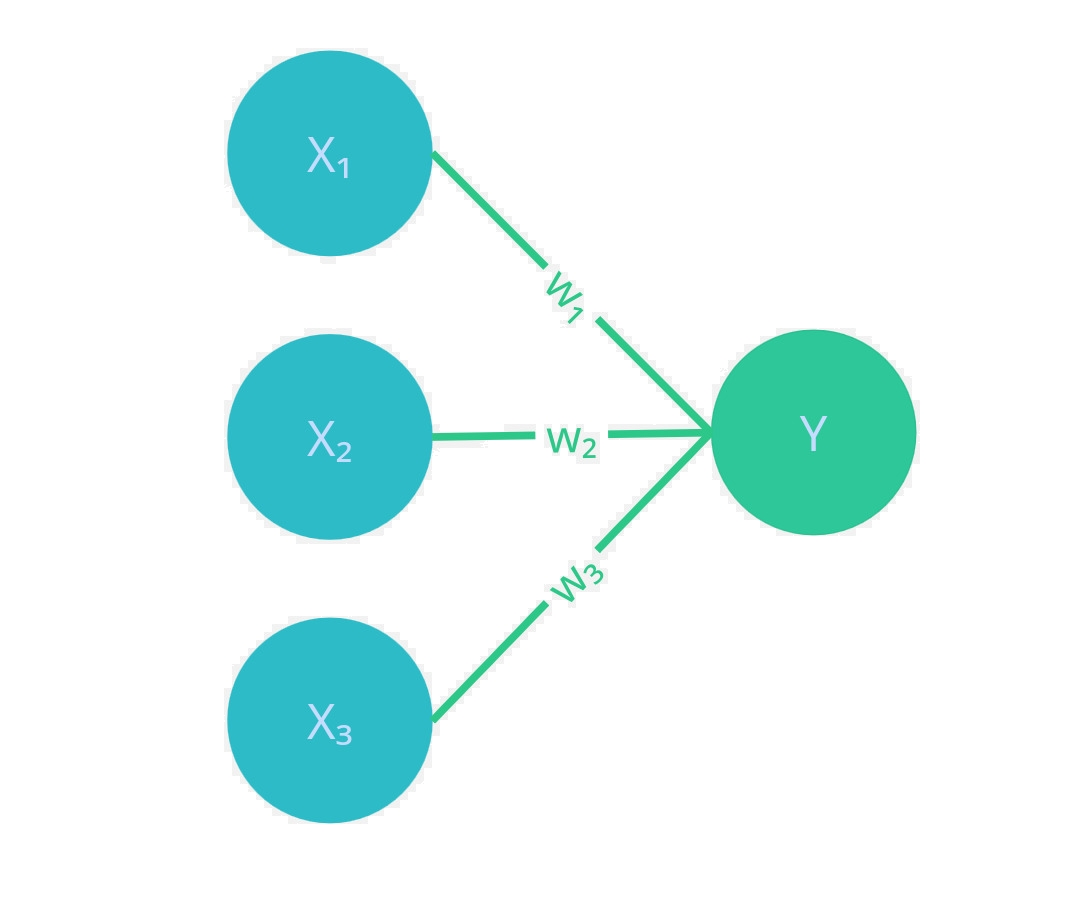
\includegraphics[width=0.9\textwidth]{input3.jpg}
    \caption{Model Representation}
\end{figure}

This is the structure of the linear regression model I will be using. It consists
of independent variables $x_1$, $x_2$, $x_3$ called inputs and a dependent variable $y$
called ouput. Inputs describe features of a particalur apartment: $x_1$ represents the
living area, $x_2$ is the construction year and $x_3$ represents the distance between
the aparment and the center of Amsterdam. The output $y$ is the price of the apartment.

A linear function that has three inputs should have three slopes, which in machine
learning are called weights $w_n$, where $w_n$ is the weight of $x_n$. Weights are constants
that are used to create the linear funciton. However, a linear function also requires
a y-intercept, which in machine learning is called a bias $b$. The whole function of y
looks like:

\[
y = w_1x_1 + w_2x_2 + w_3x_3 + b
\]

The function suggests that the price of an apartment can be calculated using those
three inputs and by multiplying them by their weights and adding a bias. The weights
and biases are constants.



\subsection{Machine Learning}

The goal of machine learning is to find the specific weights and bias that will predict
the output the most accurate.
In order to quantify the accuracy of a particular set of weights and biases a loss
function is used. A loss function $L$ has two independent variables: $y$ and $t$,
$y$ is the value predicted by the model using those weights and baises and $t$ is
the target value. There are lots of different loss functions, but I will only be
comparing three: MSE, MAE and Huber.



\subsection{Loss Functions}

\subsubsection{MSE}


\begin{figure}[H]
    \centering

    \begin{minipage}{0.4\textwidth}
        \centering
        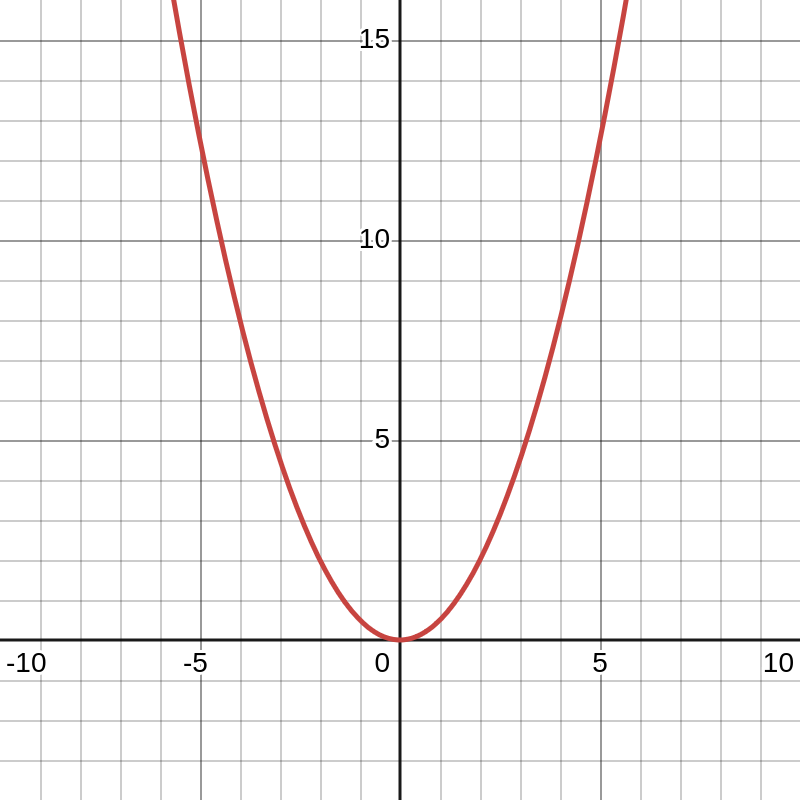
\includegraphics[width=1\textwidth]{desmos-mse.png}
        \caption{MSE loss}
        \label{single_pendulum_coordinate}
    \end{minipage}
    \hfill
    \begin{minipage}{0.55\textwidth}
        \doublespacing

        \begin{align}
        L_\mathrm{MSE} &= \frac{1}{2} (y - t) ^ 2
        \label{eq:loss_mse} \\
        L_\mathrm{MSE}' &= y - t
        \notag
        \end{align}
    \end{minipage}
\end{figure}


MSE uses squaring to create a positive difference between $y$ and $t$:
$(+5)^2 = (-5)^2$.
The half $\frac{1}{2}$ is there just to make the derivative look cleaner: $y - t$.
However, the squaring penalizes large errors disproportionately.
This could be good, as it gives more importance to cases when the model performs
the poorest, however squaring makes the learning sensitive to outliers.



\subsubsection{MAE}


\begin{figure}[H]
    \centering

    \begin{minipage}{0.4\textwidth}
        \centering
        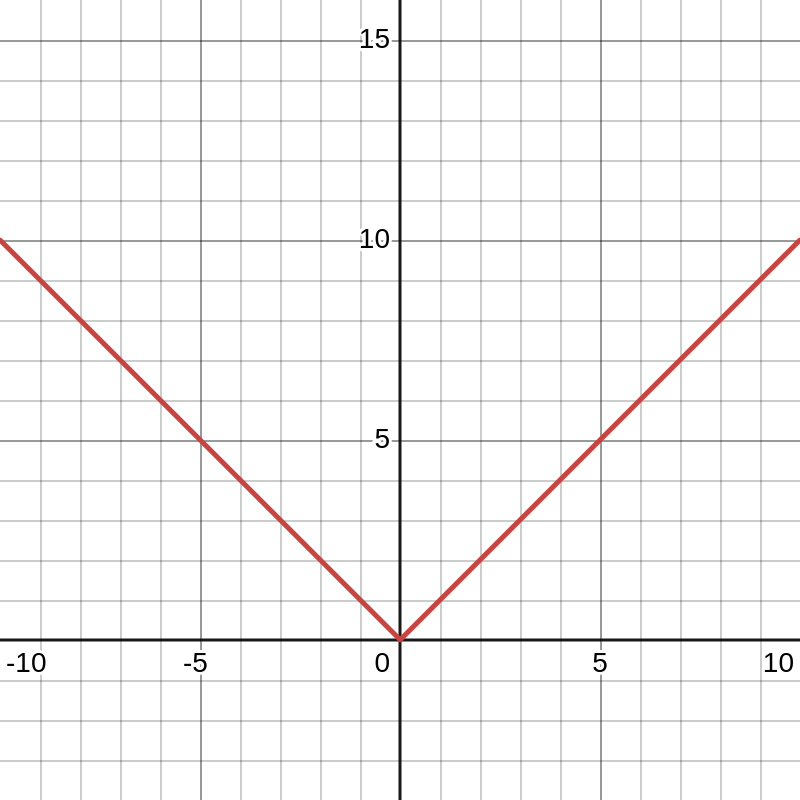
\includegraphics[width=1\textwidth]{desmos-mae.png}
        \caption{MAE loss}
    \end{minipage}
    \hfill
    \begin{minipage}{0.55\textwidth}
        \doublespacing

        \begin{align}
        L_\mathrm{MAE} &= |y - t|
        \label{eq:loss_mae} \\
        L_\mathrm{MAE}' &= \frac{|y - t|}{y - t}
        \notag
        \end{align}
    \end{minipage}
\end{figure}


MAE uses absolute value to find the error. This makes all of the erros proportionately
important. This makes it less sensitive to
outliers. However, in datasets where large errors are significant it would perform
poorly. Furthermore, this loss function is not differentiable at y = 0, as in
$\frac{|0|}{0}$ there is division by 0.


Another proof that this function is not differentiable at 0 is using limits from
both sides.

\[
\begin{split}
\text{let } &h = y - t \\
\\
\lim_{h \to 0^+} \frac{|h|}{h} &= \lim_{h \to 0^+} \frac{+h}{+h} = +1 \\
\lim_{h \to 0^-} \frac{|h|}{h} &= \lim_{h \to 0^-} \frac{+h}{-h} = -1 \\
+1 &\neq -1 \\
\lim_{h \to 0^+} L' &\neq \lim_{h \to 0^-} L' \\
\therefore \lim_{h \to 0} &\text{ does not exist}
\end{split}
\]


\subsubsection{Huber}


\begin{figure}[H]
    \centering

    \begin{minipage}{0.4\textwidth}
        \centering
        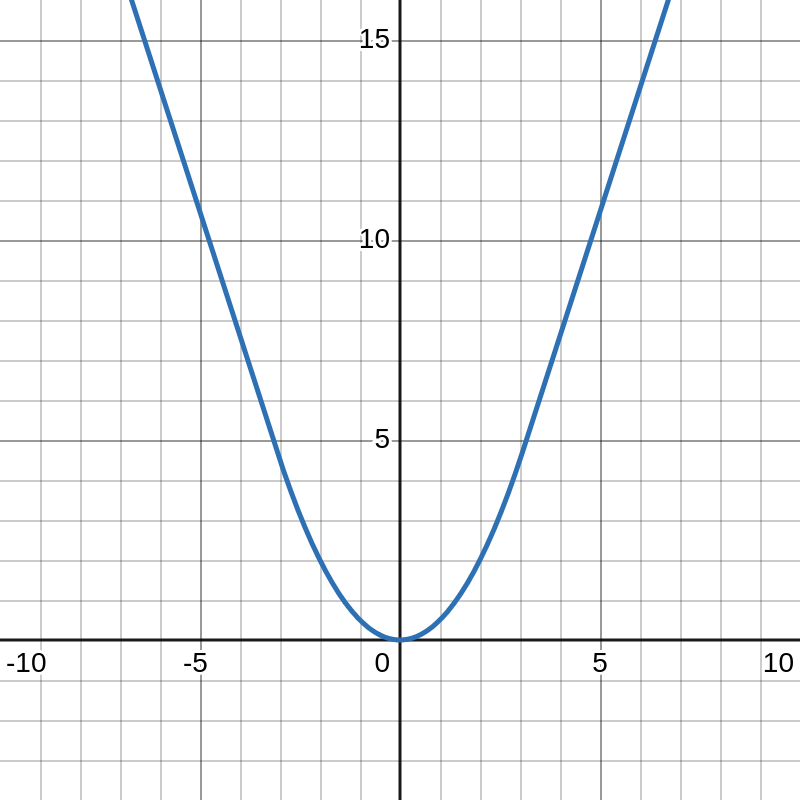
\includegraphics[width=1\textwidth]{desmos-huber.png}
        \caption{Huber loss}
    \end{minipage}
    \hfill
    \begin{minipage}{0.55\textwidth}
        \doublespacing

        \begin{align}
        L_\mathrm{Huber} &=
        \begin{cases}
        \frac{1}{2} (y - t) ^ 2, & |x| \leq \delta \\
        \delta |y - t| - \frac{1}{2} \delta^2, & |x| > \delta
        \end{cases}
        \label{eq:loss_huber} \\
        L_\mathrm{Huber}' &=
        \begin{cases}
        y - t, & |x| \leq \delta \\
        \delta \frac{|y - t|}{y - t}, & |x| > \delta
        \end{cases}
        \notag
        \end{align}
    \end{minipage}
\end{figure}



Huber takes advantages of both MSE and MAE, by combining two functions into one
piecewise, that connects at $x = \delta$. For outliers Huber uses MAE, which makes
their impact less significant. On the other hand, MSE makes the other data points
have different importances depending on the errors' magnitude. The only problem is
finding the most efficient $\delta$. There isn't a straight forward way of finding
the constant. Usually values like $\delta = 0.5, 1.0, 1.345, 2.0, 5.0$ are used.
In order to find the best coefficient for my data I have tested the values above.



\subsection{Gradient Descent}

\subsubsection{Visualize}

Gradient descent is the what calculates a particular weight or bias during the
machine learning. As shown on the diagram below, we could plot the loss function,
in this case MSE is used, and drop the weight on a random point. Now, after calculating
the gradient of the loss function we could change the weight in the correct direction
to get closer to the local minimum. On this example only one weight varies, and
every other weight and bias are fixed. In the actual machine learning, which will
be done further, every weight and bias will have its own curve, in which they
all will be adjusted to approach the minimum of the function simultaneously.




\begin{figure}[H]
    \centering

    \begin{minipage}{0.49\textwidth}
        \centering
        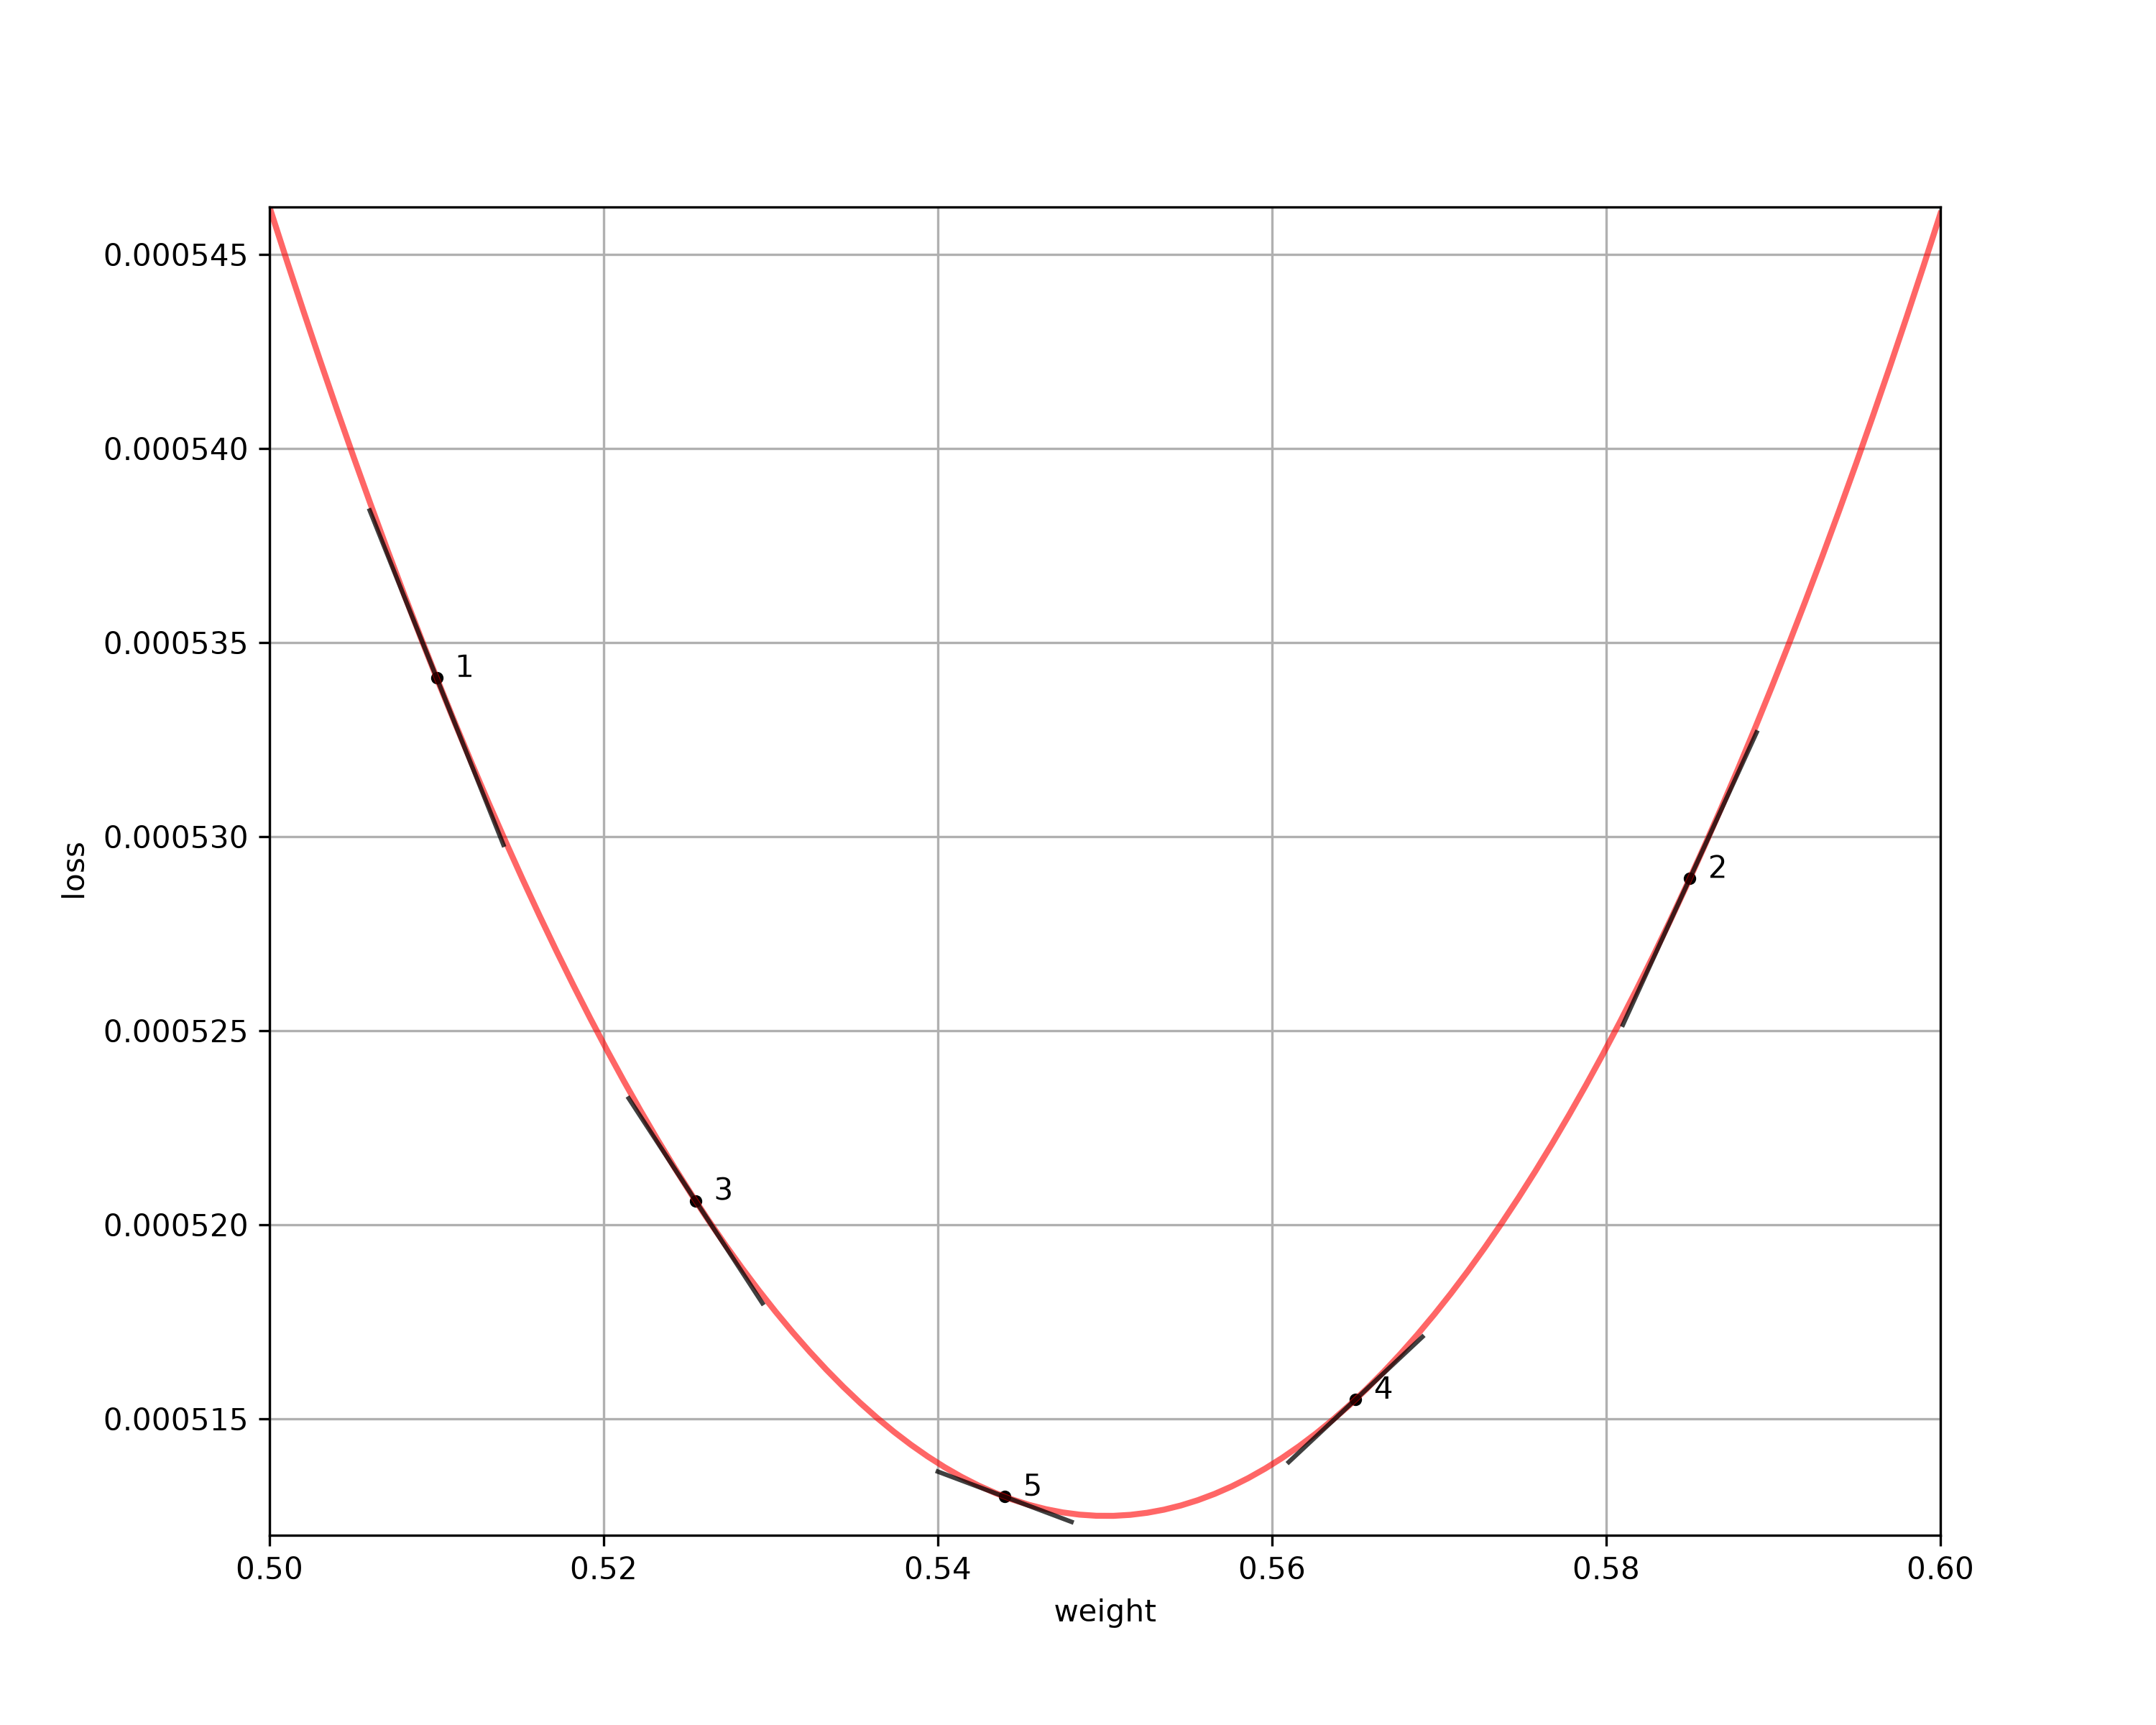
\includegraphics[width=\textwidth]{graph_jumps_dots_labels.png}
        \caption{Gradient Descent}
    \end{minipage}
    \hfill
    \begin{minipage}{0.49\textwidth}
        \centering
        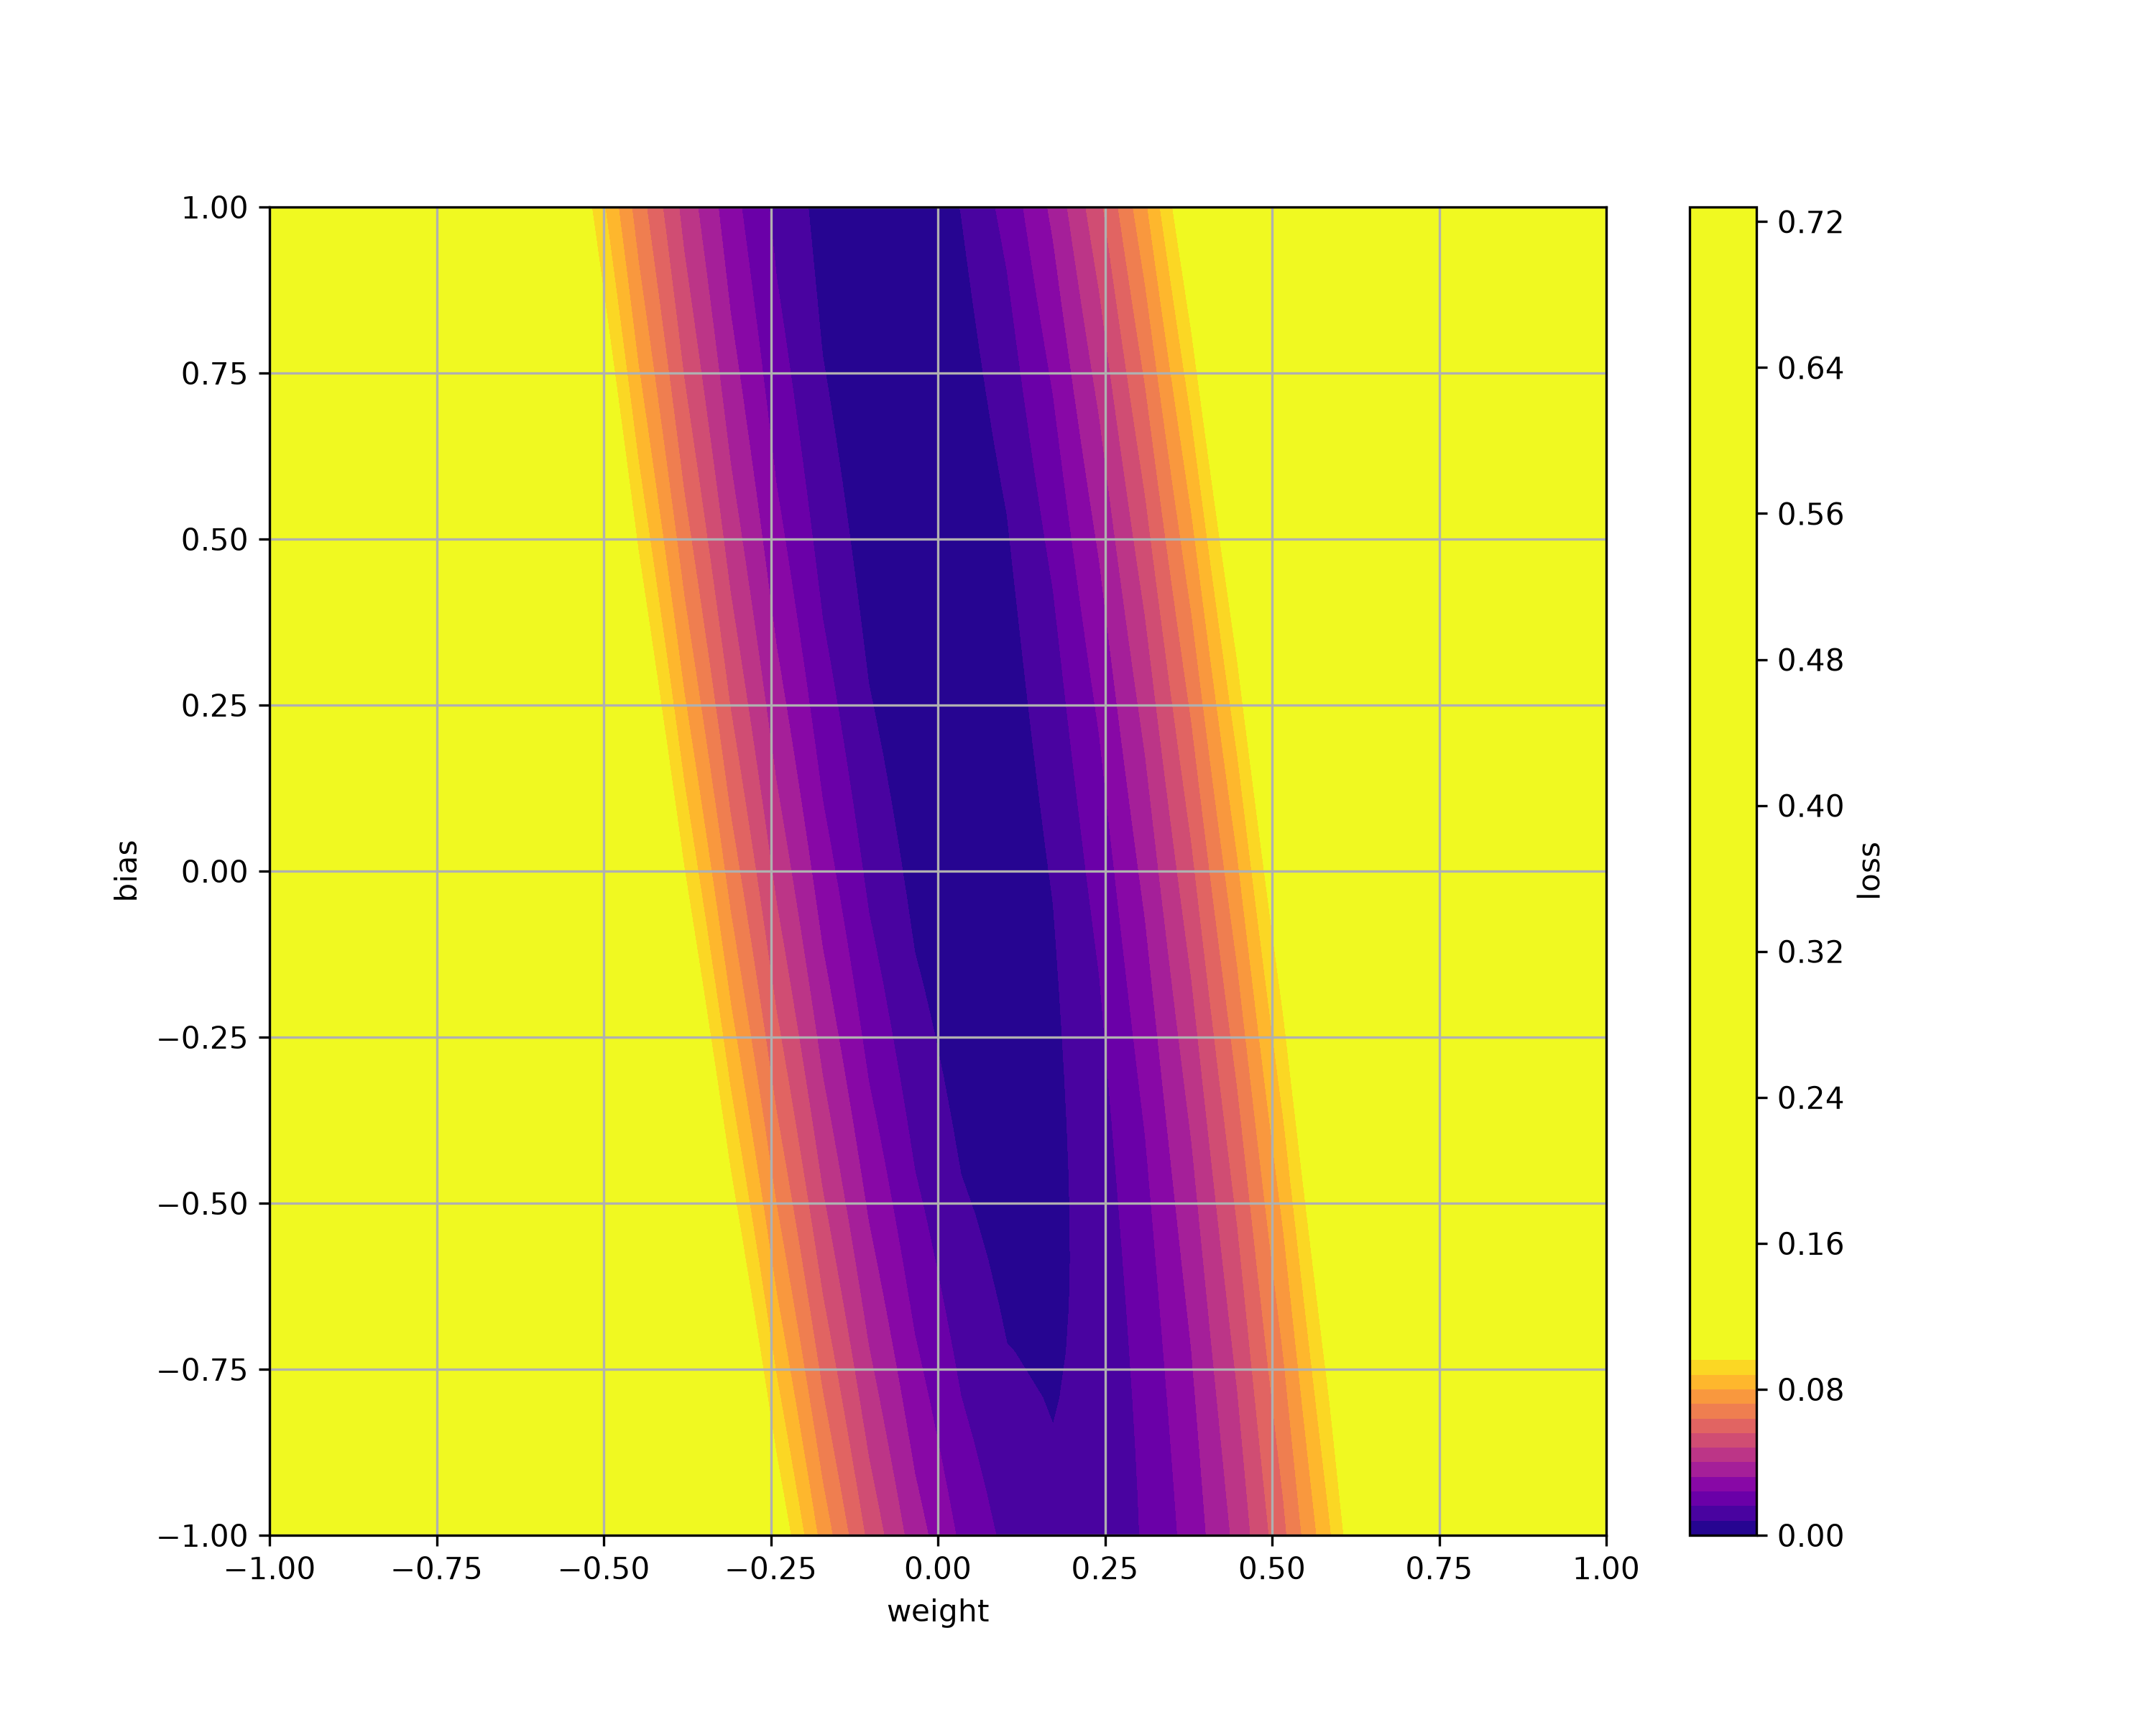
\includegraphics[width=\textwidth]{graph_weight_bias_loss_sharp.png}
        \caption{Countour Map}
    \end{minipage}
\end{figure}




% On the graph, the bias is fixed so that it is easier to visualize. Now, to minimize the
% loss, gradient descent is used. It works by finding the gradients of weight(s) and bias(es)
% (here it is fixed) and then moving in the direction of the steepest gradient, achieving the
% minimum of the function.

% At the very start, the weight is random; it is around 0.51. The gradient is calculated and
% subtracted from the weight, because we want to minimize the loss. The same thing is repeated
% as many times as possible to achieve the smallest loss, and the gradient ensures that the loss
% is decreasing.


To visualize how gradient descent would look while multiple variables are changing,
I have computed this contour map where $y$, $t$ are fixed and $w_2$ and $w_3$ are
random constants, and depending on how $w_1$ and $b$ are tweaked (by the axis)
the loss is changing (indicated with the color). (I have picked only two variables
because it would be almost impossible to visualize a five dimensional
function like $L_\mathrm{MSE}$ even with $y$ and $t$ fixed).

We can see the purple spots on the diagram which represent the minimums or
the lower loss areas. The gradient descent should, if set up properly, tweak
$w_1$ and $b$ that way that the loss will move to those areas.

% This diagram illustrates the loss function with parameters of weight and bias, instead of
% fixing one of them. The x and y axis are weight and bias, respectively, and the color
% represents loss as shown on the right side with the colorbar.

% \[
% L(w, b) = \frac{1}{2}{((wx + b) - t)} ^ 2
% \]

% Apart from showing the dependency of loss on weight and bias, this diagram also highlights
% the limitation of the learning method. Gradient decent finds the local minimum of loss
% function, however this particular local minimum that the model would converge to might
% not be the global minimum.


\subsubsection{Differentiate to find the Gradients}

The gradient of weight in this graph is just the partial derivative of the loss by the weight.
I will start of with writing down all of the equations we have:

\[
\begin{split}
L(y, t) &= \frac{1}{2}{(y - t)} ^ 2 \\
y &= w_1x_1 + w_2x_2 + w_3x_3 + b
\end{split}
\]

In order to derive further I will have to use partial derivatives. A partial derivative
is a type of derivative that amplies to multi dimensional/variable functions when
we have to figure out the rate of change of this function in one particular dimension.
To partially derive a function I have to treat all of the other variables as
constants just for the derivative.
First I derive MSE loss with respect to $y$, so treat $t$ as a constant:

\begin{equation}
\frac{\partial L}{\partial y} = y - t
\label{eq:dLdy}
\end{equation}

Now if I want to partially derive $y$ with respects to $w_1$, to see how
the answer changes with the first weight (this is the one dimension):

\[
\begin{split}
\frac{\partial y}{\partial w_1} &=
\frac{\partial y}{\partial w_1} (w_1 x_1) +
\frac{\partial y}{\partial w_1} (w_2 x_2) +
\frac{\partial y}{\partial w_1} (w_3 x_3) = \\
&= x_1 + 0 + 0 = x_1
\end{split}
\]

Now using the chain rule $\frac{du}{dv} = \frac{du}{dn} \times \frac{dn}{dv}$,
I can combine two derivatives and find the gradient of $w_1$ with respect to $L$:


\begin{equation}
\begin{split}
\frac{\partial L}{\partial w_1} &=
\frac{\partial L}{\partial y} \times \frac{\partial y}{\partial w_1} = \\
&= (y - t) {\times} x_1
\end{split}
\label{eq:dLdw}
\end{equation}


This needs to be done with every other weight and the bias:

\[
\begin{split}
\frac{\partial L}{\partial w_2} =
\frac{\partial L}{\partial y} \times \frac{\partial y}{\partial w_2} &=
(y - t) \times x_2 \\
\frac{\partial L}{\partial w_3} =
\frac{\partial L}{\partial y} \times \frac{\partial y}{\partial w_3} &=
(y - t) \times x_3 \\
\frac{\partial L}{\partial b} =
\frac{\partial L}{\partial y} \times \frac{\partial y}{\partial b} &=
(y - t)
\end{split}
\]


\subsubsection{Tweak the Weights and Biases}


This is how the model knows in what direction to change the weights/bias and how
important it is too change a weight/bias to reduce the loss. To change a
weight/bias we could just substract the derivative from the weight:

\[
\begin{split}
\text{let } h &= \text{weight $w_n$ or bias $b$} \\
h &= h - \frac{\partial L}{\partial h}
\end{split}
\]

However, the derivative might be too big, and the weight/bias could change too much. This could
cause instability, as the weight could overshoot all the time, and it might never reach the
minimum. To address this a learning rate constant is introduced - $\eta$. The derivative is
multiplied by it too ensure that the steps are small so that the minimum is achieved no matter
what. The formula for weight change becomes:

\begin{equation}
h = h - \frac{\partial L}{\partial h} \times \eta
\label{eq:w_change}
\end{equation}

$\eta$ is usually somewhere around 0.1 to 0.001. This is done to every weight/bias
bias during the machine learning process. So for example, this would be the formula
for the first weight changing with learning rate $\eta$ of 0.1, using MSE loss:


\[
\begin{split}
w_1 &= w_1 - \frac{\partial L}{\partial w_1} \times 0.1 \\
w_1 &= w_1 - (y - t) \times x_1 \times 0.1
\end{split}
\]



One of the things I have not mentioned yet is where I got the $x$ and $t$ from. As I said $x$
is the living area, and $t$ is the price of an apartment. I have collected data from funda.nl
and I only picked the apartments that are in Amsterdam and that are for sale in July of 2026.
In total, I have collected around 4500 apartments with their respective prices and features.

Because the function does calculation of only one apartment at a time, I took average of all
losses for each apartment with a certain weight and bias and that is what is being presented
on the previous graphs. That is why I have not used $x$ nor $t$ as arguments for functions $y$
and $L$, for the process of learning it is treated as a constant. The weight and bias are the
independent variables that must be changed. After the model has finished its learning and,
therefore, has constant weight and bias, the function will become $y(x) = wx + b$ and $x$
will be the independent variable again.


% \subsection{Not Normalized}

% Another thing that must be done for a model to work is normalization of inputs and outputs.
% Here is an example, that will explain the importance of normalization:

% I will take learning rate as 0.001, it is 10 times less than I normally would use because
% this will illustrate the influence of normalization clearer.

% An apartment that is located at 1061 AV Amsterdam has price is 930 000 {\euro} and it has living
% area of 108 $m^2$. Let $w$ be 8700 and $b$ be 348, those are values that achieve a decent
% amount of accuracy for this example. The function is:

% \[
% y(x) = 8700 {\times} x + 348
% \]

% $x$ is the living area, so it is 108 $m^2$. $y$ is the predicted price:

% \[
% y(x) = 8700 {\times} 108 + 348 = 939 948 \text{ \euro}
% \]

% $t$ is the target price, so it is 930 000 {\euro}. Using $t$ and $y$ we can now
% calculate the loss:

% \[
% \begin{split}
% L(x) &= \frac{1}{2}{(y(x) - 930000)} ^ 2 \\
% \Rightarrow L(108) &= \frac{1}{2}{(939948 - 930000)} ^ 2 = \\
% &= 4.95 \times 10^{7}
% \end{split}
% \]


% Now we calculate the gradient decent:


% \[
% \begin{split}
% {\partial}L/{\partial}w &= (y - t) {\times} x = (939948 - 930000) {\times} 108 = 1074.4 \times 10^{3} \\
% w &= w - {\partial}L/{\partial}w {\times} \eta = (8700 - 1074.4 \times 10^{3}) {\times} 0.001 = 7625.616 \\
% {\partial}L/{\partial}b &= (y - t) = (939948 - 930000) = 9.9 \times 10^{3} \\
% b &= b - {\partial}L/{\partial}b {\times} \eta = (348 - 9.9 \times 10^{3}) {\times} 0.001 = 338.052
% \end{split}
% \]

% And calculate the loss again with new weight and bias:

% \[
% \begin{split}
% y(108) &= 7625.616 {\times} 108 + 338.052 = \\
% &= 823 904.58 \text{ \euro} \\
% L(108) &= \frac{1}{2}{(y - t)} ^ 2 = \frac{1}{2}{(823904.58 - 930000)} ^ 2 = \\
% &= 562.8 \times 10^{7} \\
% \end{split}
% \]

% The new loss is significantly larger than the first one:
% $4.95 \times 10^{7} < 562.8 \times 10^{7}$
% Although the gradient descent should have decreased the loss, it overshoot instead.
% The initial weights and biases were definitely wrong, as the first prediction
% was around 54 \euro. However, because of the huge inputs - 108 and the target outputs
% - 930 000, the gradients skyrocketed: $1074.4 \times 10^{3}$, $9.9 \times 10^{3}$. Although the
% learning rate was small - 0.001, smaller then normal, the weight and bias still overshot. This experiment can be
% repeated with any other weights and most of the time, the derivative will overshoot and the
% model will not minimize the loss function and therefore will not learn.

\subsection{Normalization}

Another thing that must be done for a model to work is normalization of inputs and outputs.
Normalization is the process of fitting a set of values into the range between
0 to 1.

\begin{equation}
x_{\mathrm{norm}} = \frac{x_{\mathrm{raw}} - x_{\min}}{x_{\max} - x_{\min}}
\end{equation}


Where $x_{\mathrm{raw}}$ is the value to be normalized; $x_{\min}$ and $x_{\max}$
are the minimum and maximum values of the same type in the dataset; $x_{\mathrm{norm}}$
is the normalized value in the range 0 - 1.


This is done for every input: price, living area and distance, and the ouput: the
price of the apartment.
Normalization will ensure that weights are also in a small range, usually from -1 to 1,
rarely might reach -2, or 2.

For my data the min and max for prices and living areas are respectively:

\[
\begin{split}
x_1 &= 19 - 500 \text{ $m^2$} \\
x_2 &= 1507 - 2028 \text{ year} \\
x_3 &= 0.07 - 9.98 \text{ km} \\
y &= 189 - 9850 \text{ k\euro}
\end{split}
\]

Also, I divide the price by $10^{3}$, keeping it in thousand of euros (k\euro).
This makes the numbers clearer and potentially has a small impact on the training,
as the data is shrank by 1000 and the difference between prices is lower.

I will repeat the same example but with normalized values now, the weight and biases are
also chosen so that the function is somewhat accurate:

\[
\begin{split}
w &= 0.5 \\
b &= -0.03 \\
\\
x &= 108 \text{ $m^2$} \\
t &= 930k \text{ \euro} \\
\\
x_{\mathrm{norm}} &= (x - x_{\min}) / (x_{\max} - x_{\min}) \\
&= (108 - 19) / (500 - 19) = 0.185 \\
t_{\mathrm{norm}} &= (t - t_{\min}) / (t_{\max} - t_{\min}) \\
&= (930 - 189) / (9850 - 189) = 0.0767
\end{split}
\]


Since all of the values will be normalized from now on, I will not use the \_norm suffix.

\[
\begin{split}
y &= 0.5 {\times} x - 0.03 = 0.5 {\times} 0.185 - 0.03 = 0.0625 \\
L &= \frac{1}{2}{(y - t)} ^ 2 = \frac{1}{2}{(0.0625 - 0.0767)} ^ 2 = 1.006 {\times} 10^{-4}
\end{split}
\]

\[
\begin{split}
{\partial}L/{\partial}w &= (y - t) {\times} x = (0.0625 - 0.0767) {\times} 0.185 = -2.62 {\times} 10^{-3} \\
w &= w - {\partial}L/{\partial}w {\times} \eta = 0.5 - -0.00262 {\times} 0.1 = 0.50026 \\
\\
{\partial}L/{\partial}b &= (y - t) = 0. 0625 - 0.0767 = -1.42 {\times} 10^{-2} \\
b &= b - {\partial}L/{\partial}b {\times} \eta = -0.03 - -0.0142 {\times} 0.1 = -0.0286
\end{split}
\]

\[
\begin{split}
y &= wx + b = 0.50026 {\times} 0.185 - 0.0286 = 0.064 \\
L &= \frac{1}{2}{(y - t)} ^ 2 = \frac{1}{2}{(0.064 - 0.0767)} ^ 2 = 0.809 {\times} 10^{-4}
\end{split}
\]


As can be seen here the loss decreased from $1.00 {\times} 10^{-4}$ to
$0.81 {\times} 10^{-4}$. Normalization allows for a more stable learning process and
less overshooting during the gradient descent. Moreover, normalization helps with weights
and biases initialization, as we can assume that they are going to be most frequently
around -1.0 to 1.0. On the other hand, without normalization the weights might go to
thousands like in the last example. The diagram below shows how centered the blue
graph (normalized data) to the zero compared to the red graph (not normalized data).
Furthermore, the gradient is much less steep for the blue graph, which again shows that
the gradient descent will be more smooth and less overshooting.

\begin{figure}[H]
    \centering
    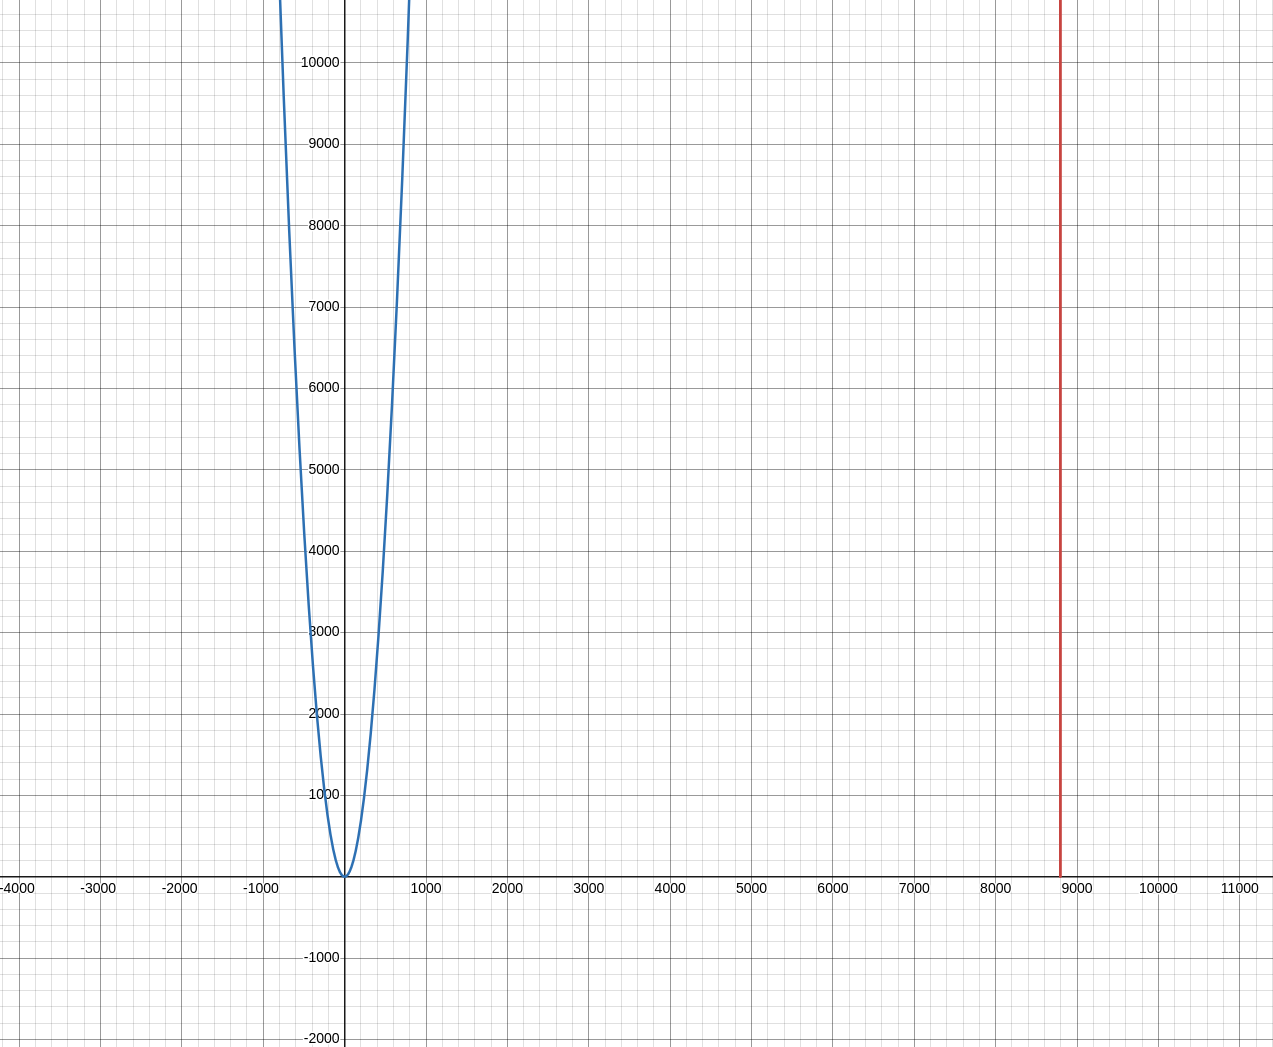
\includegraphics[width=0.9\textwidth]{orig_vs_norm.png}
    \caption{Normalized vs not Normalized}
\end{figure}


\subsection{Learning Process}

I have a few thousand apartments data from which my model must learn.
The term epoch is introduced at this point, which refers to a single, complete
pass of the entire training dataset through the model. In this case, gradient
descent will be done for each apartment in the dataset. $x$ is the living area,
and $t$ is the respective price for the apartments. This will make the model
find the middle ground for weight and bias to minimize the loss across
all the apartments. For a model to minimize loss as much as possible, numerous
epochs are done. Depending on the length of the dataset this number can range,
but I will be doing around 100-1000 epochs.

As I mentioned earlier, the dataset includes around 4500 entries; it is exactly
4577 apartments. I have separated the data into training and test datasets. The
training entries are used to train the model, in the process mentioned above.
On the other hand, the test dataset is used to test the accuracy of predictions
of the model. The test process illustrates how good the model performs on
apartments it has never seen before. To separate the dataset into training and
test datasets, I will be using a 0.95 ratio - 4348 and 229 entries, respectively.


\section{Experiment}

Here is the model I have trained on my dataset with the structure $y = wx + b$,
learning rate 0.01 and 1000 epochs.
Blue points are the entries from the dataset, and the red dots are the predictions
made by the model.


\begin{figure}[H]
    \centering
    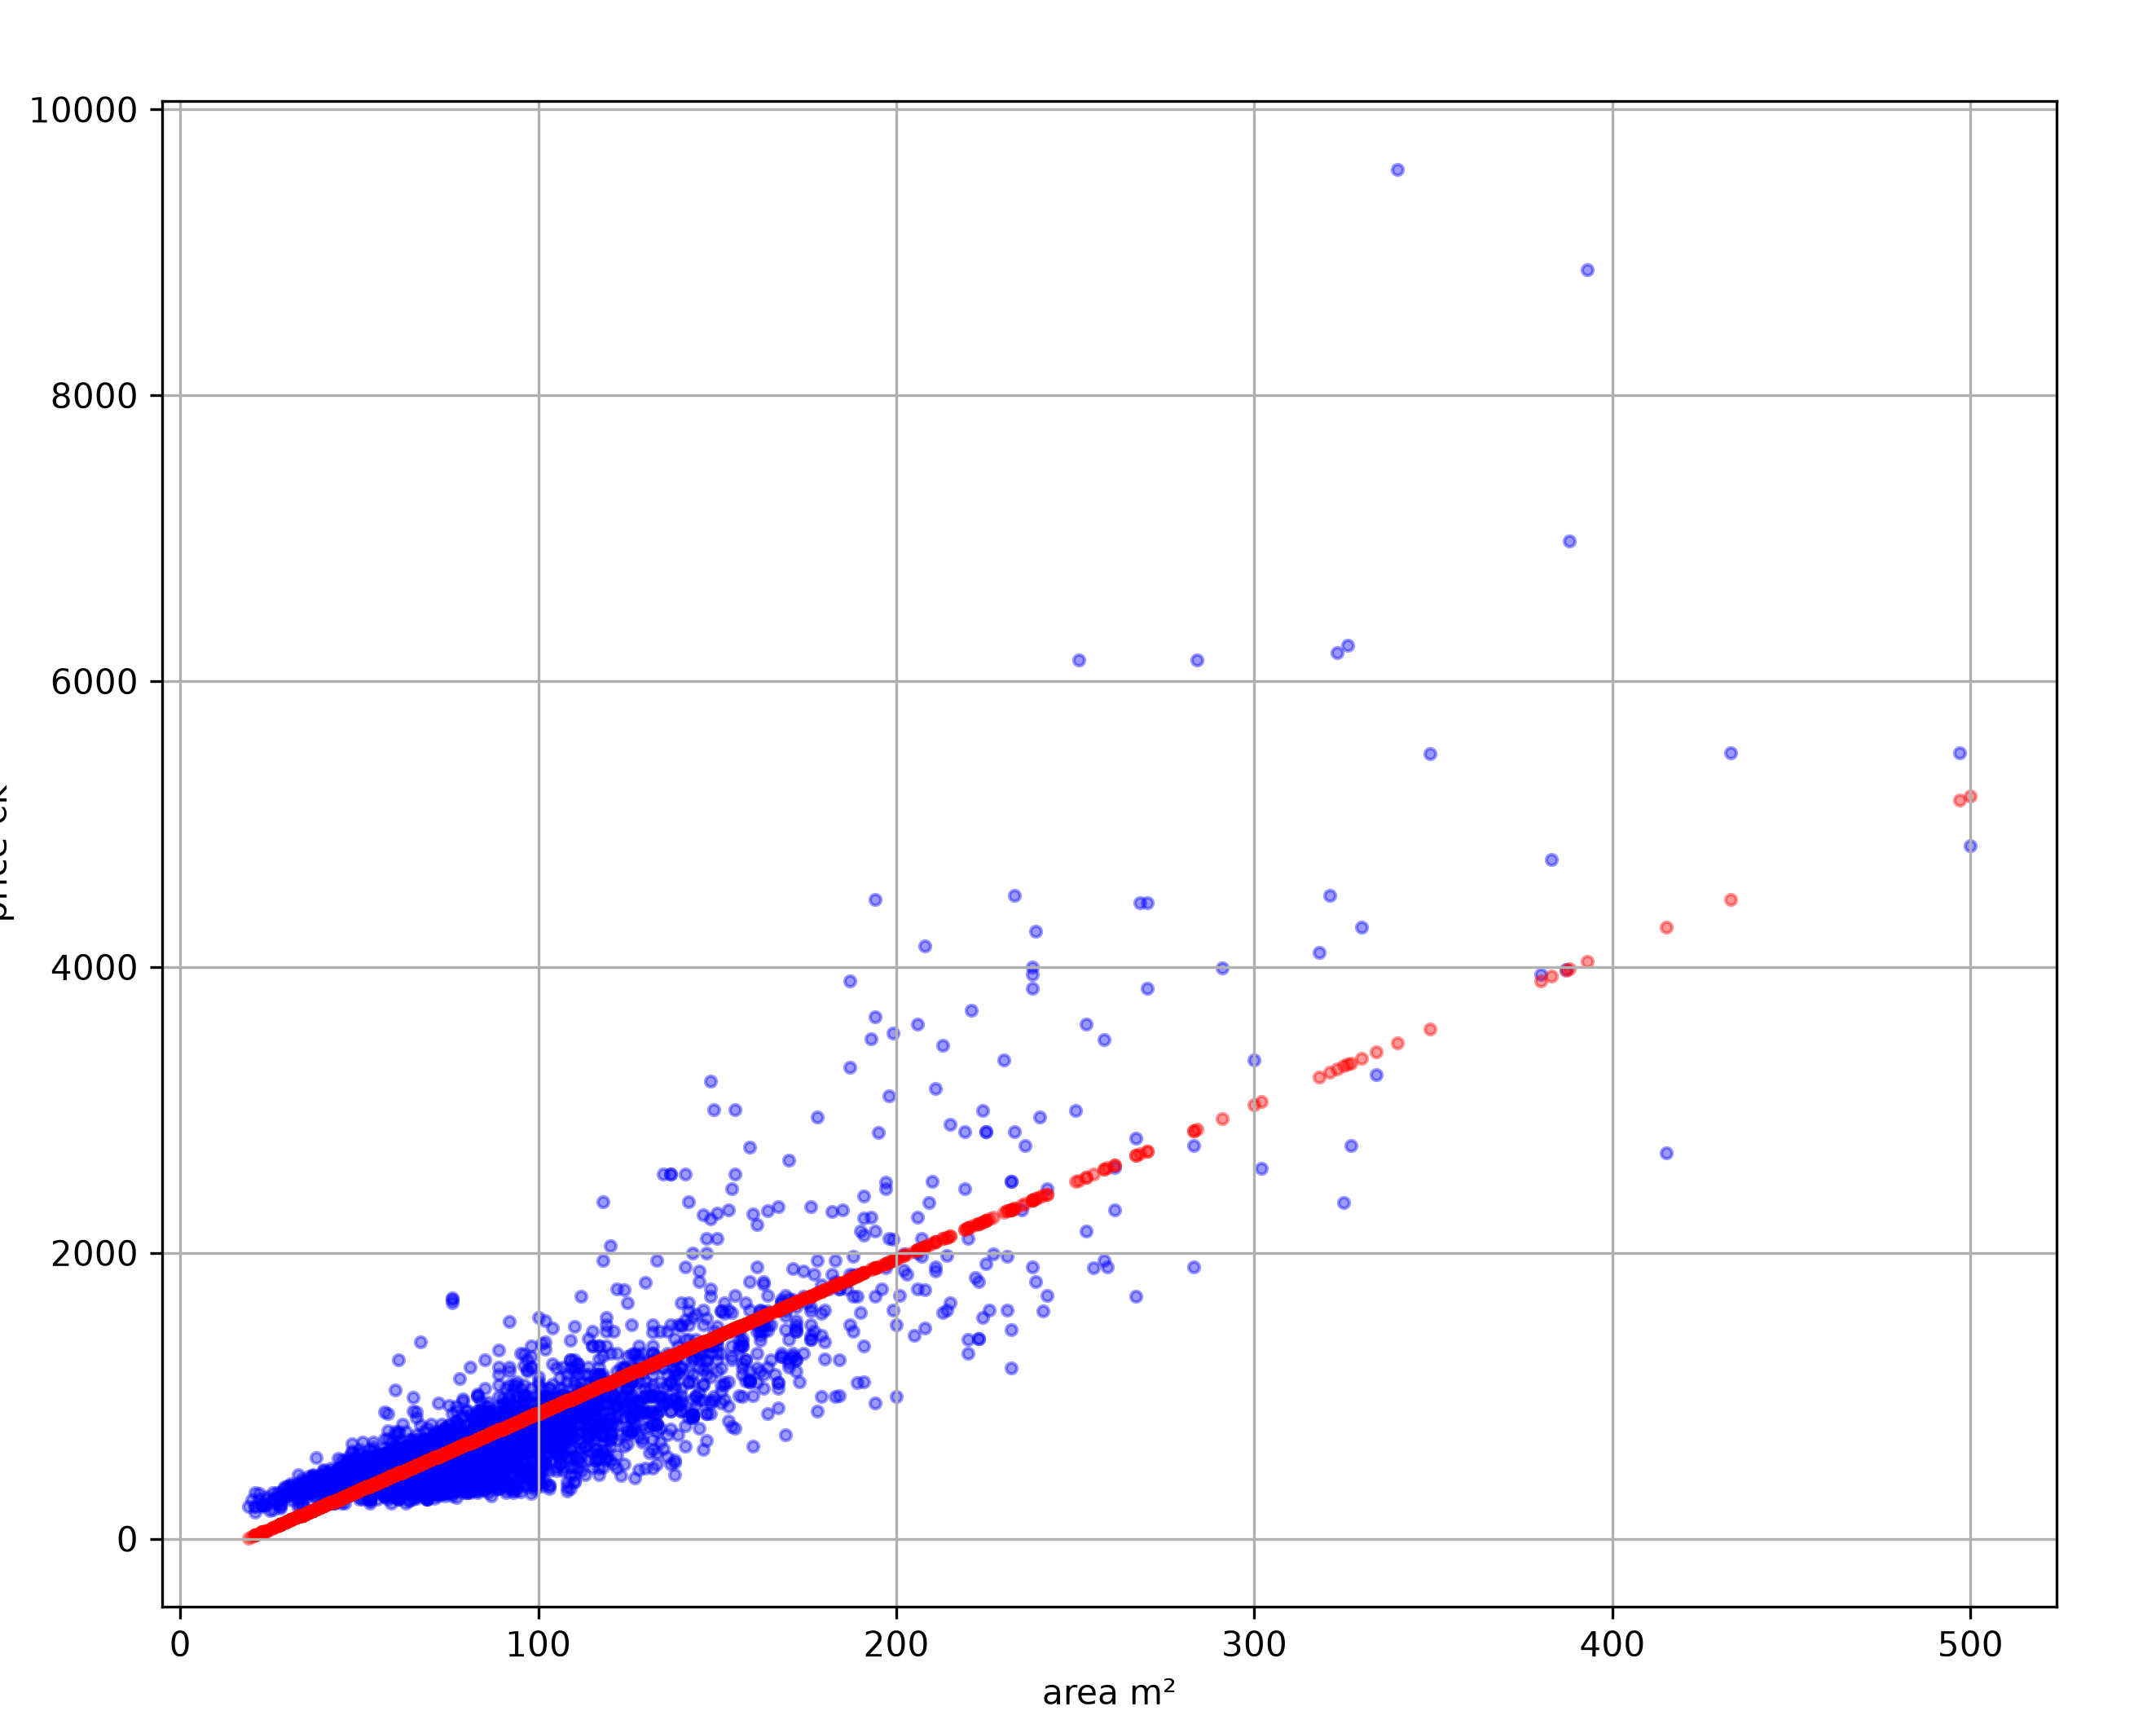
\includegraphics[height=0.4\textheight]{graph_area.png}
    \caption{Model Results}
\end{figure}


\begin{figure}[H]
    \centering
    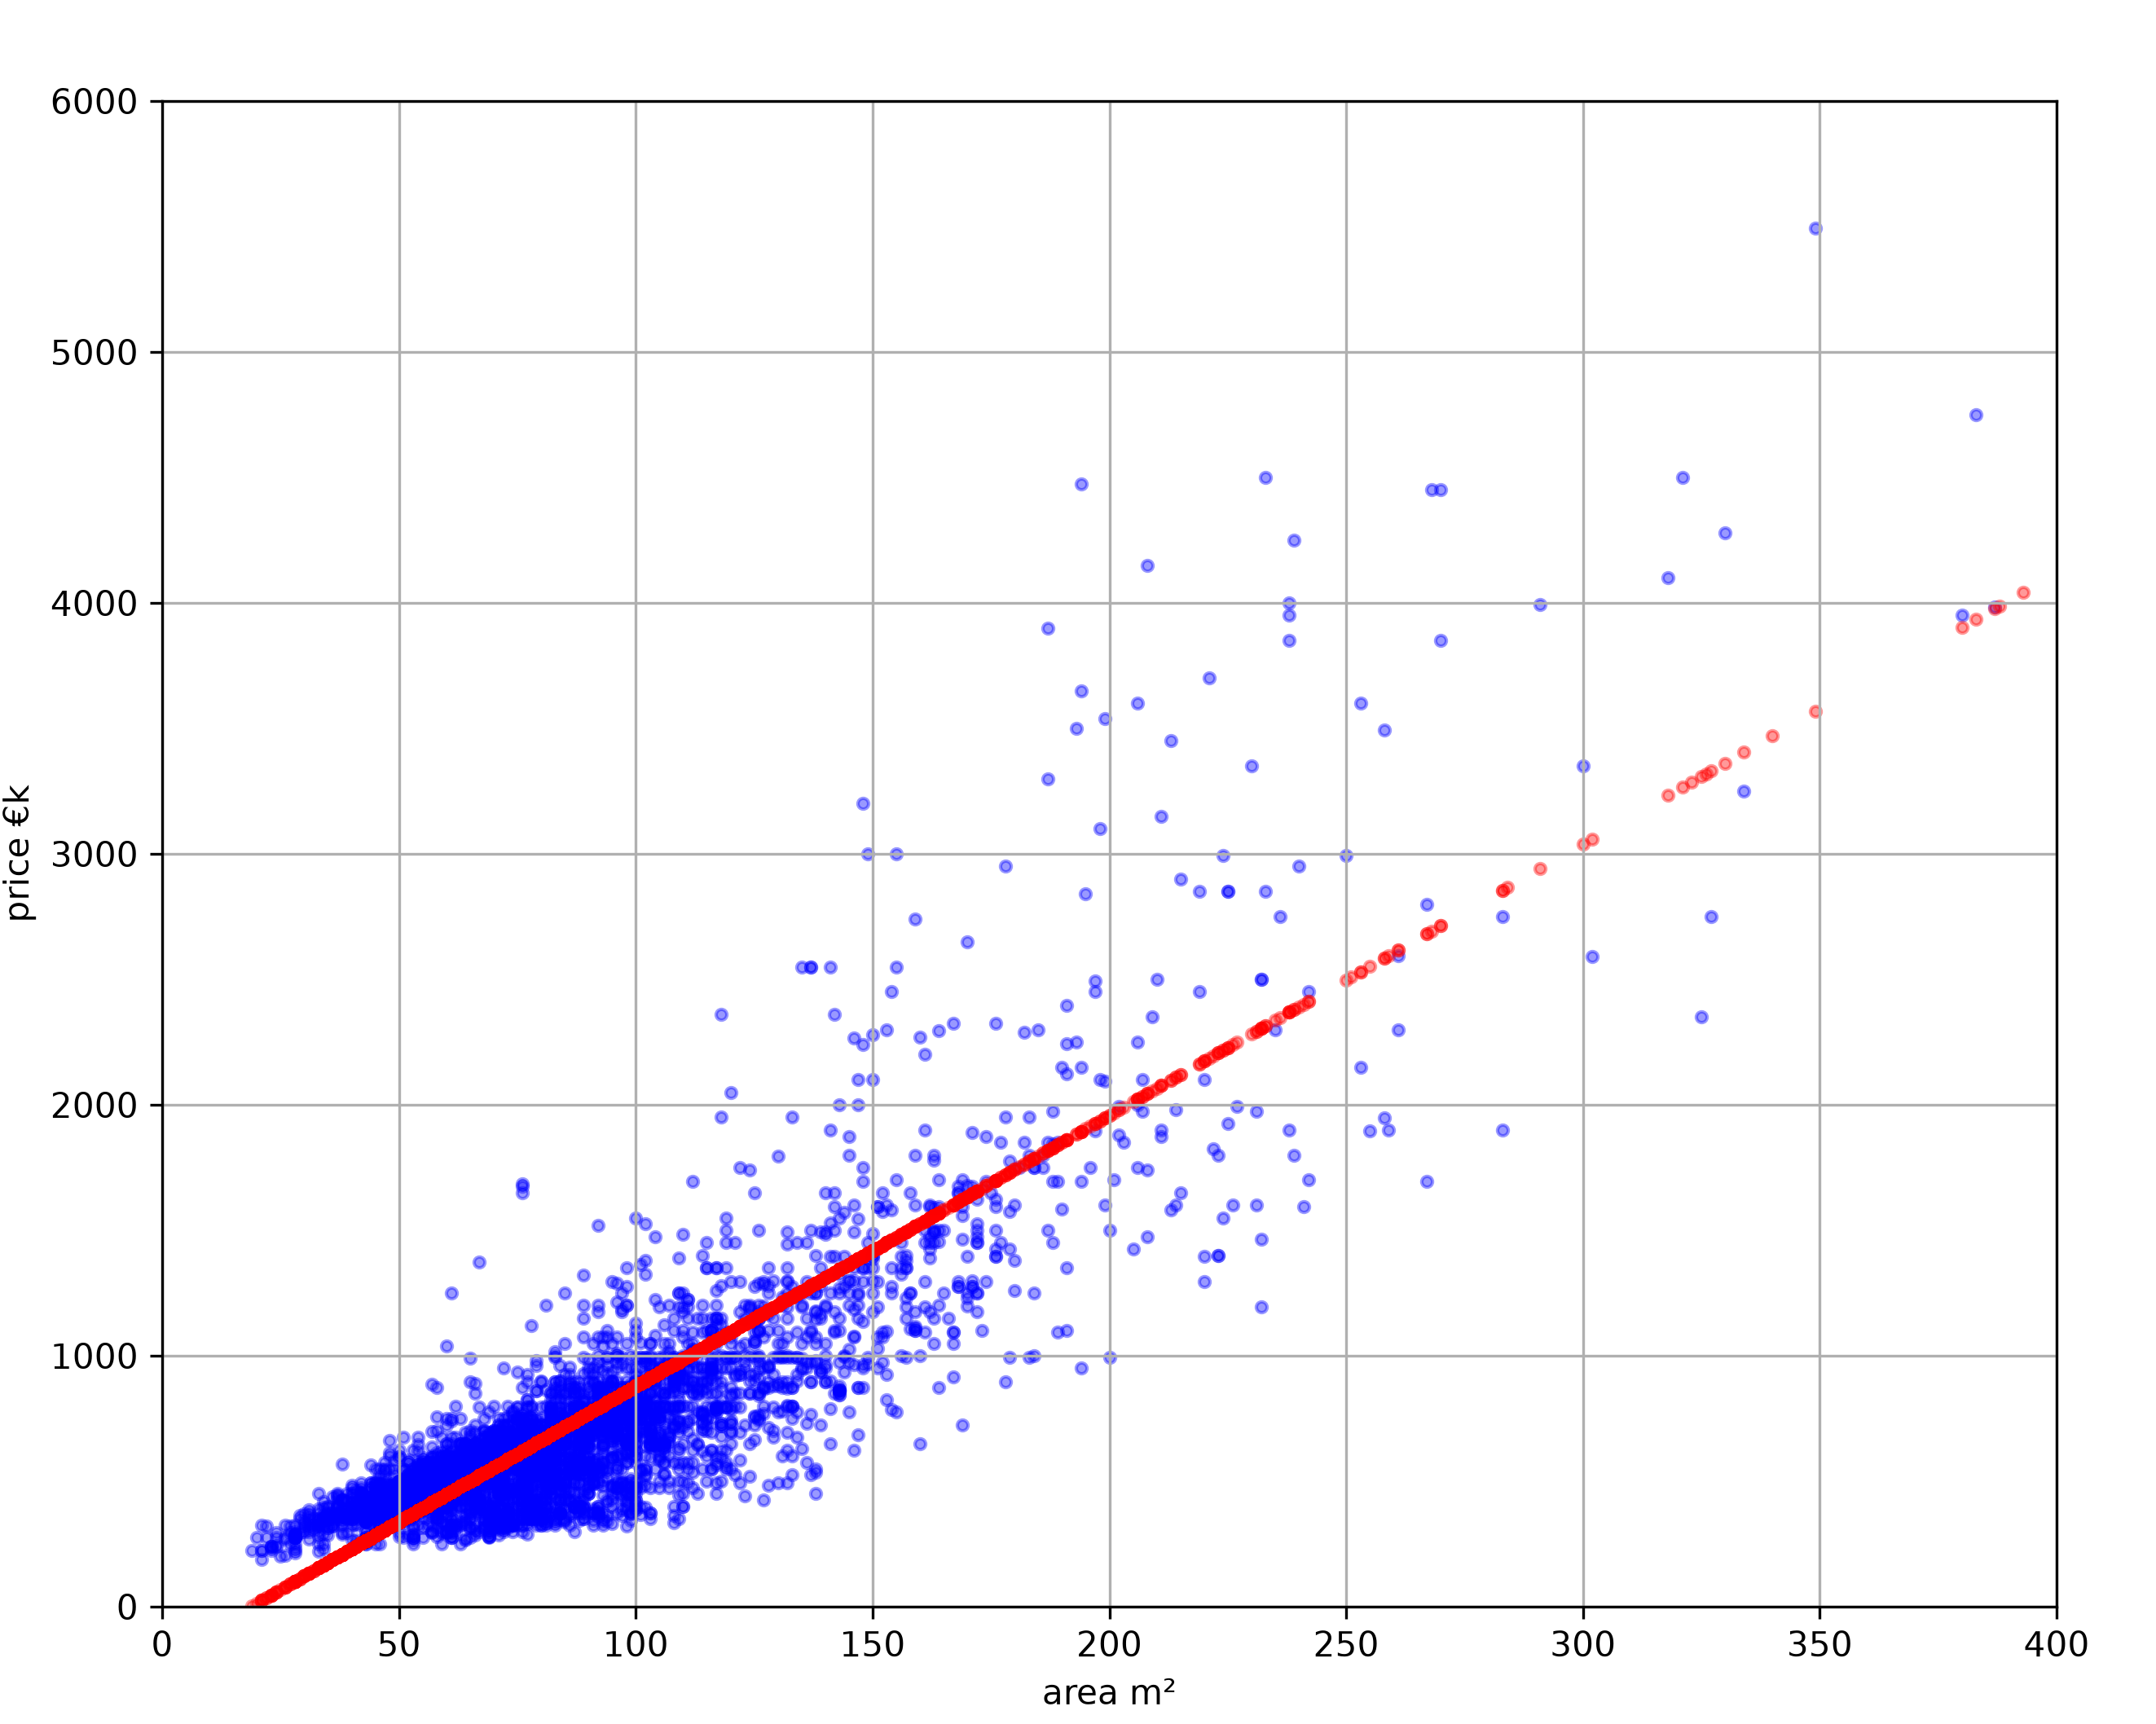
\includegraphics[height=0.4\textheight]{graph_area_zoom.png}
    \caption{Model Results Without Outliers}
\end{figure}


This model has converged its weight and bias values to around 0.553 and -0.0197,
respectively. This achieved the loss of $4.798 {\times} 10^{-4}$. I want to remind you that in
previous example I achieved less loss, $0.81 {\times} 10^{-4}$ because the loss was calculated
across one entry which practically has a certain weight and bias that achieves
0 loss. $y = wx + b$ where $y$ and $x$ are constants means that there are infinitely many
solutions.

On the other hand, here are 4500 entries that are impossible to cover with a linear
equation like this. This line that my model has learned is just the best perfect line.
Furthermore, the blue dots are arranged in a mostly chaotic way with a tendency of the
price increasing as the area increases. This suggests that only area is not enough to
fully predict price of house.

Nevertheless, this model can predict housing, although accuracy is limited. I can build
a function according to the weight and bias I got:

\[
y(x) = 0.5497 {\times} x - 0.0186
\]

Let's test it on this example:

\[
\begin{split}
\text{Area } &- \text{ 79 $m^2$} \\
\text{Target price } &- \text{700k {\euro}}
\end{split}
\]

First normalize the data:

\[
x = \frac{79 - 19}{500 - 19} = 0.1247
\]

Use the function:

\[
\begin{split}
y(x) &= 0.5497 {\times} x - 0.0186 \\
{\Rightarrow} \: y(0.1247) &= 0.5497 {\times} 0.1247 - 0.0186 = 0.0499
\end{split}
\]

Now we can denormalize $y$ by rearranging the normalization function:

\begin{equation}
\begin{split}
y_{\mathrm{norm}} &= \frac{y - y_{\min}}{y_{\max} - y_{\min}} \\
y_{\mathrm{norm}} {\times} (y_{\max} - y_{\min}) &= y - y_{\min} \\
y &= y_{\mathrm{norm}} {\times} (y_{\max} - y_{\min}) + y_{\min} \\
\end{split}
\label{eq:y_norm}
\end{equation}

\[
y = 0.0493 {\times} (9850 - 189) + 189 = 671.46
\]

The target was 700k and the model predicted 671.46k which is not
too bad for a model that only has the information about living
area.

To assess how good this model actually is, this process must be done for
more than one apartment. I put this model through my test dataset, with the
results I got I can calculate the mean absolute error $\mathrm{MAE}$ and mean
percentage absolute error $\mathrm{MAPE}$.

\begin{align}
{\mathrm{MAE}}  = \frac{1}{n} \sum_{i=1}^{n} |y_i - t_i|
\label{eq:MAE} \\
{\mathrm{MAPE}} = \frac{100\%}{n} \sum_{i=1}^{n} \frac{|y_i - t_i|}{t_i}
\label{eq:MAPE}
\end{align}

I got $\mathrm{MAE} = 162.0k$ and $\mathrm{MAPE} = 25.5\%$. Here are few other examples of
predictions this model has made:


\begin{table}[h]
\centering
\begin{tabular}{c|c|c|c|c|c|c}
Target $t$ (k {\euro})
& 359.0 & 450.0 & 475.0 & 650.0 & 685.0 & 880.0 \\
\hline
Predicted $y$ (k {\euro})
& 454.1 & 357.5 & 378.9 & 604.3 & 840.4 & 1205.3 \\
\end{tabular}
\end{table}


3.749e-04 is the least loss I was able to get while using only one feature of the
apartments.


\section{Building network with 3 inputs}

\[
y(x_1, x_2, x_3) = w_1x_1 + w_2x_2 + w_3x_3 + b
\]

From here I can get all the derivatives necessary, using derivatives from Equations
~\ref{eq:dLdy}, ~\ref{eq:dLdw} and ~\ref{eq:dLdb}. As always, while deriviving partially,
I treat other variables as constants:


\[
\begin{split}
{\partial}L/{\partial}w_1 &= (y - t) * x_1 \\
{\partial}L/{\partial}w_2 &= (y - t) * x_2 \\
{\partial}L/{\partial}w_3 &= (y - t) * x_3 \\
{\partial}L/{\partial}b &= y - t
\end{split}
\]


\begin{figure}[H]
    \centering
    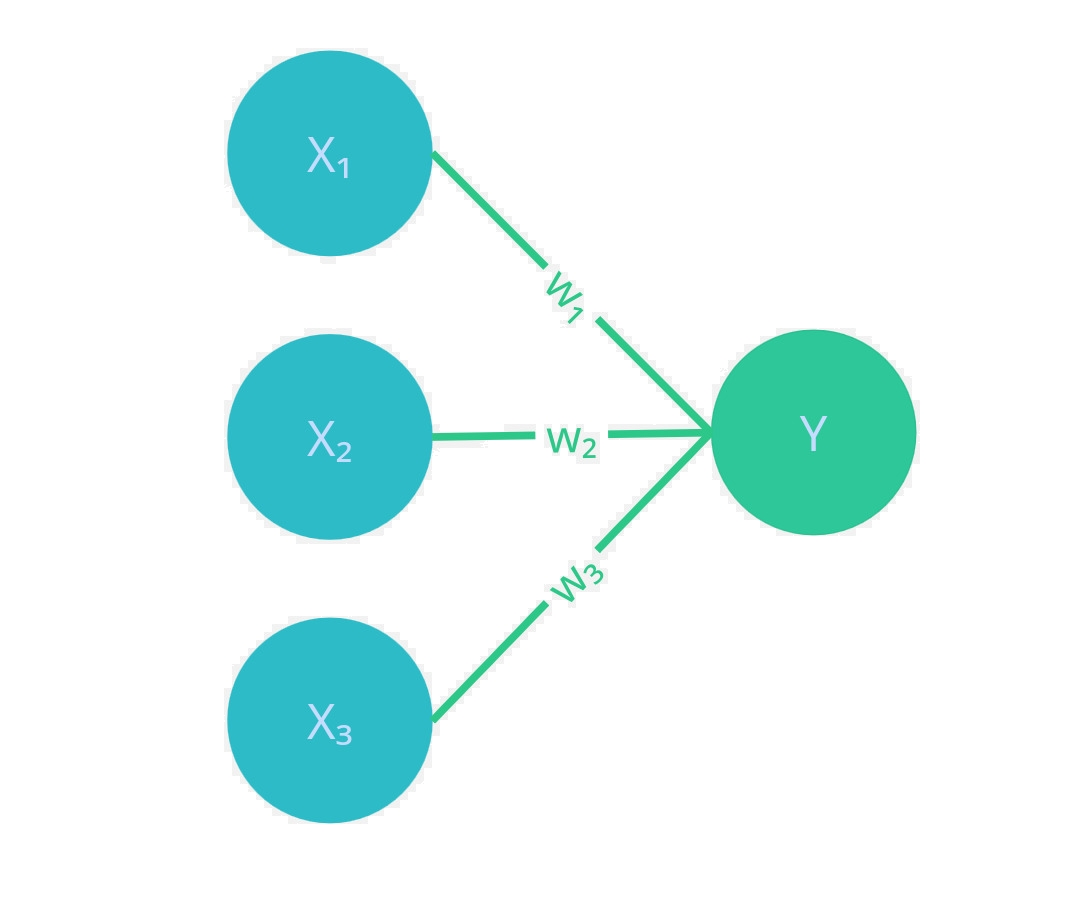
\includegraphics[width=0.9\textwidth]{input3.jpg}
    \caption{3 Input Model}
\end{figure}


With this I can train a model for 1000 epochs. These are the weights and the bias,
the model has converged to:

\[
\begin{split}
w_1 &= 0.5429 \\
w_2 &= -0.0077 \\
w_3 &= -0.0534 \\
b &= 0.0072
\end{split}
\]


Let's test it on the previous example:

\[
\begin{split}
\text{Area } &- \text{ 79 $m^2$} \\
\text{Year } &- \text{2005} \\
\text{Distance} &- \text{1.806 km} \\
\text{Target price} &- \text{700k {\euro}}
\end{split}
\]

Normalize inputs:

\[
\begin{split}
x_1 = \frac{79 - 19}{500 - 19} = 0.1247 \\
x_2 = \frac{2005 - 1507}{2028 - 1507} = 0.9559 \\
x_3 = \frac{1.806 - 0.07}{9.98 - 0.07} = 0.1752
\end{split}
\]

Calculate:

\[
\begin{split}
y(0.1247, 0.9559, 0.1752) &= 0.5429 {\times} 0.1247 + \\
&+ -0.0077 {\times} 0.9559 + \\
&+ -0.0534 {\times} 0.1752 + \\
&+ 0.0072 = \\
&= 0.0582
\end{split}
\]

Denormalize according to Equation~\ref{eq:y_norm}:

\[
y {\times} (9850 - 189) + 189 = 751.34
\]

This time the model overshot the price, but this model has achieved the best
results with the test dataset on average making $3.01 {\times} 10^{-4}$ loss, and having
the $\mathrm{MAE}$ and $\mathrm{MAPE}$ of 130.2 and 18.3\%, respectively.

Here are some other results:

\begin{table}[h]
\centering
\begin{tabular}{c|c|c|c|c|c|c}
Target $t$ (k {\euro})
& 359.0 & 450.0 & 475.0 & 650.0 & 685.0 & 880.0 \\
\hline
Predicted $y$ (k {\euro})
& 317.0 & 467.3 & 354.6 & 587.3 & 890.9 & 1105.1 \\
\end{tabular}
\end{table}

\subsection{Influence of Distance on Price}

Just like last time we can measure the influence of each input by the absolute
values of their weights:

\[
\begin{split}
| w_1 | = 0.5429 \\
| w_2 | = 0.0077 \\
| w_3 | = 0.0534
\end{split}
\]

We can see that the most influential input is still area, but the importance of
construction year dramatically fell from 0.05 to 0.008, and the influence of
distance is in middle of two other inputs.

Here is how the distribution of distance across the dataset looks like,
(I have removed few outliers again):

\begin{figure}[H]
    \centering
    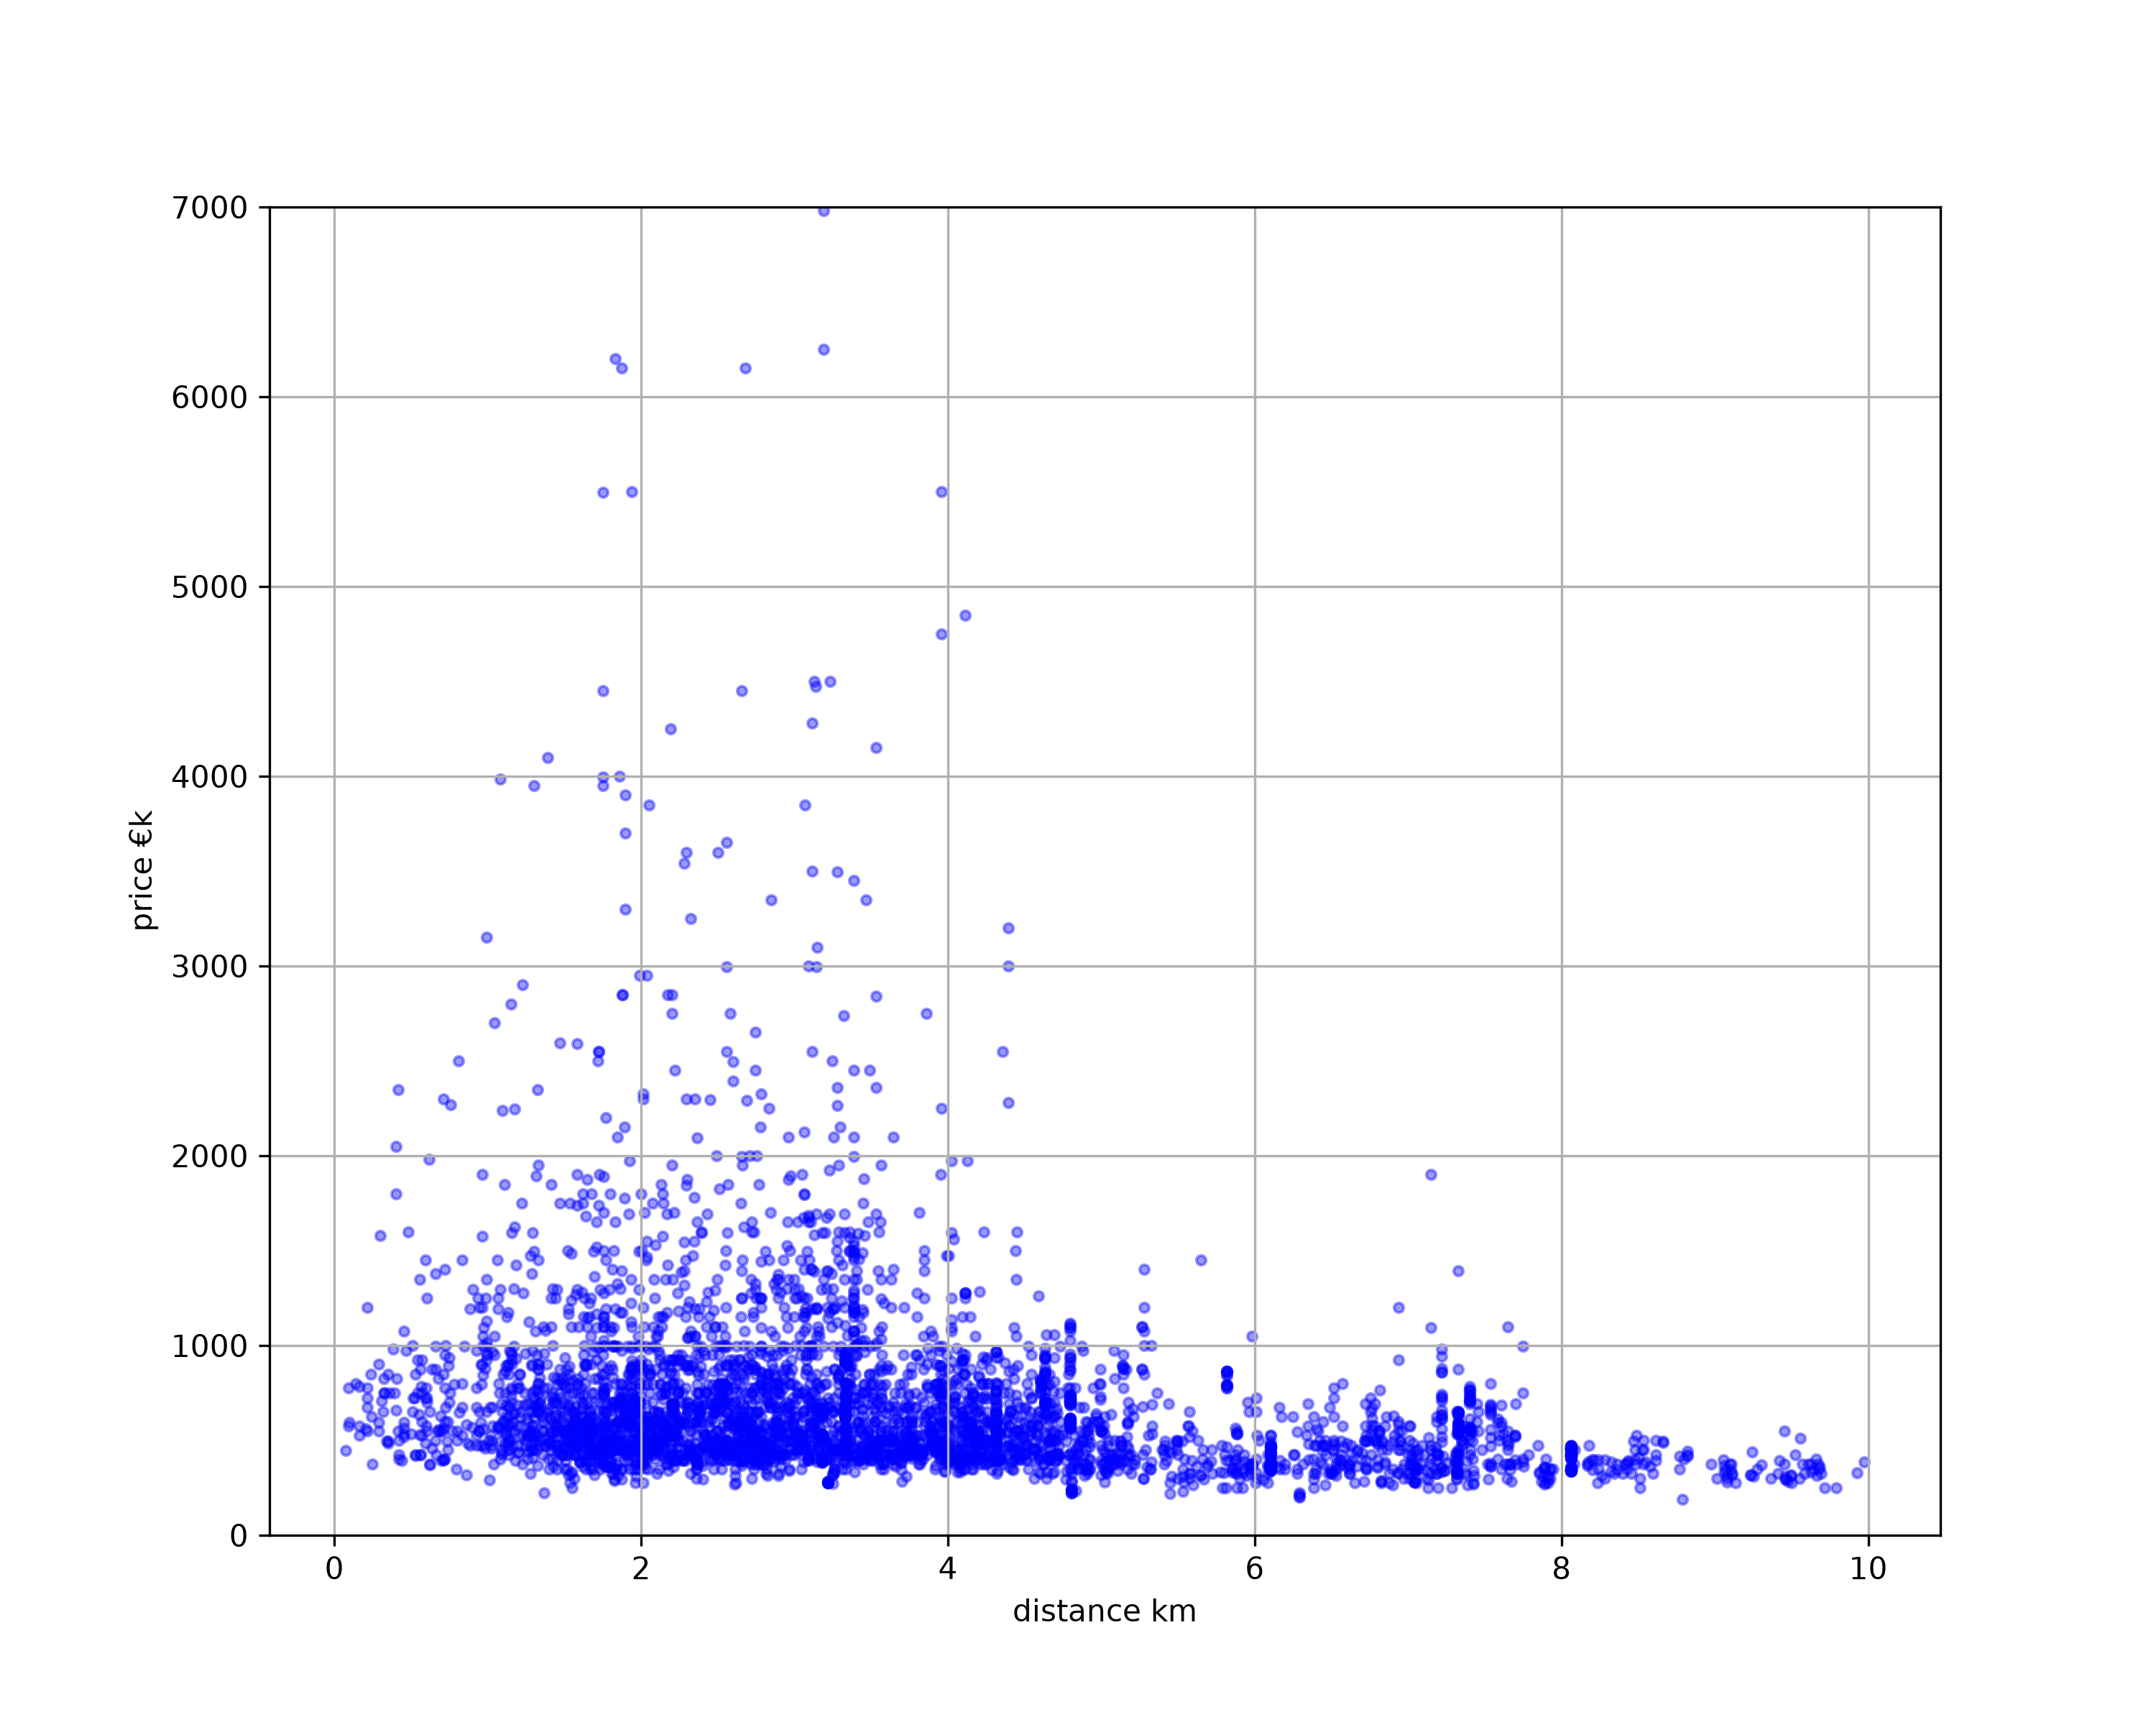
\includegraphics[width=0.9\textwidth]{graph_distance.png}
    \caption{Distance against Price Data}
\end{figure}

\begin{figure}[H]
    \centering
    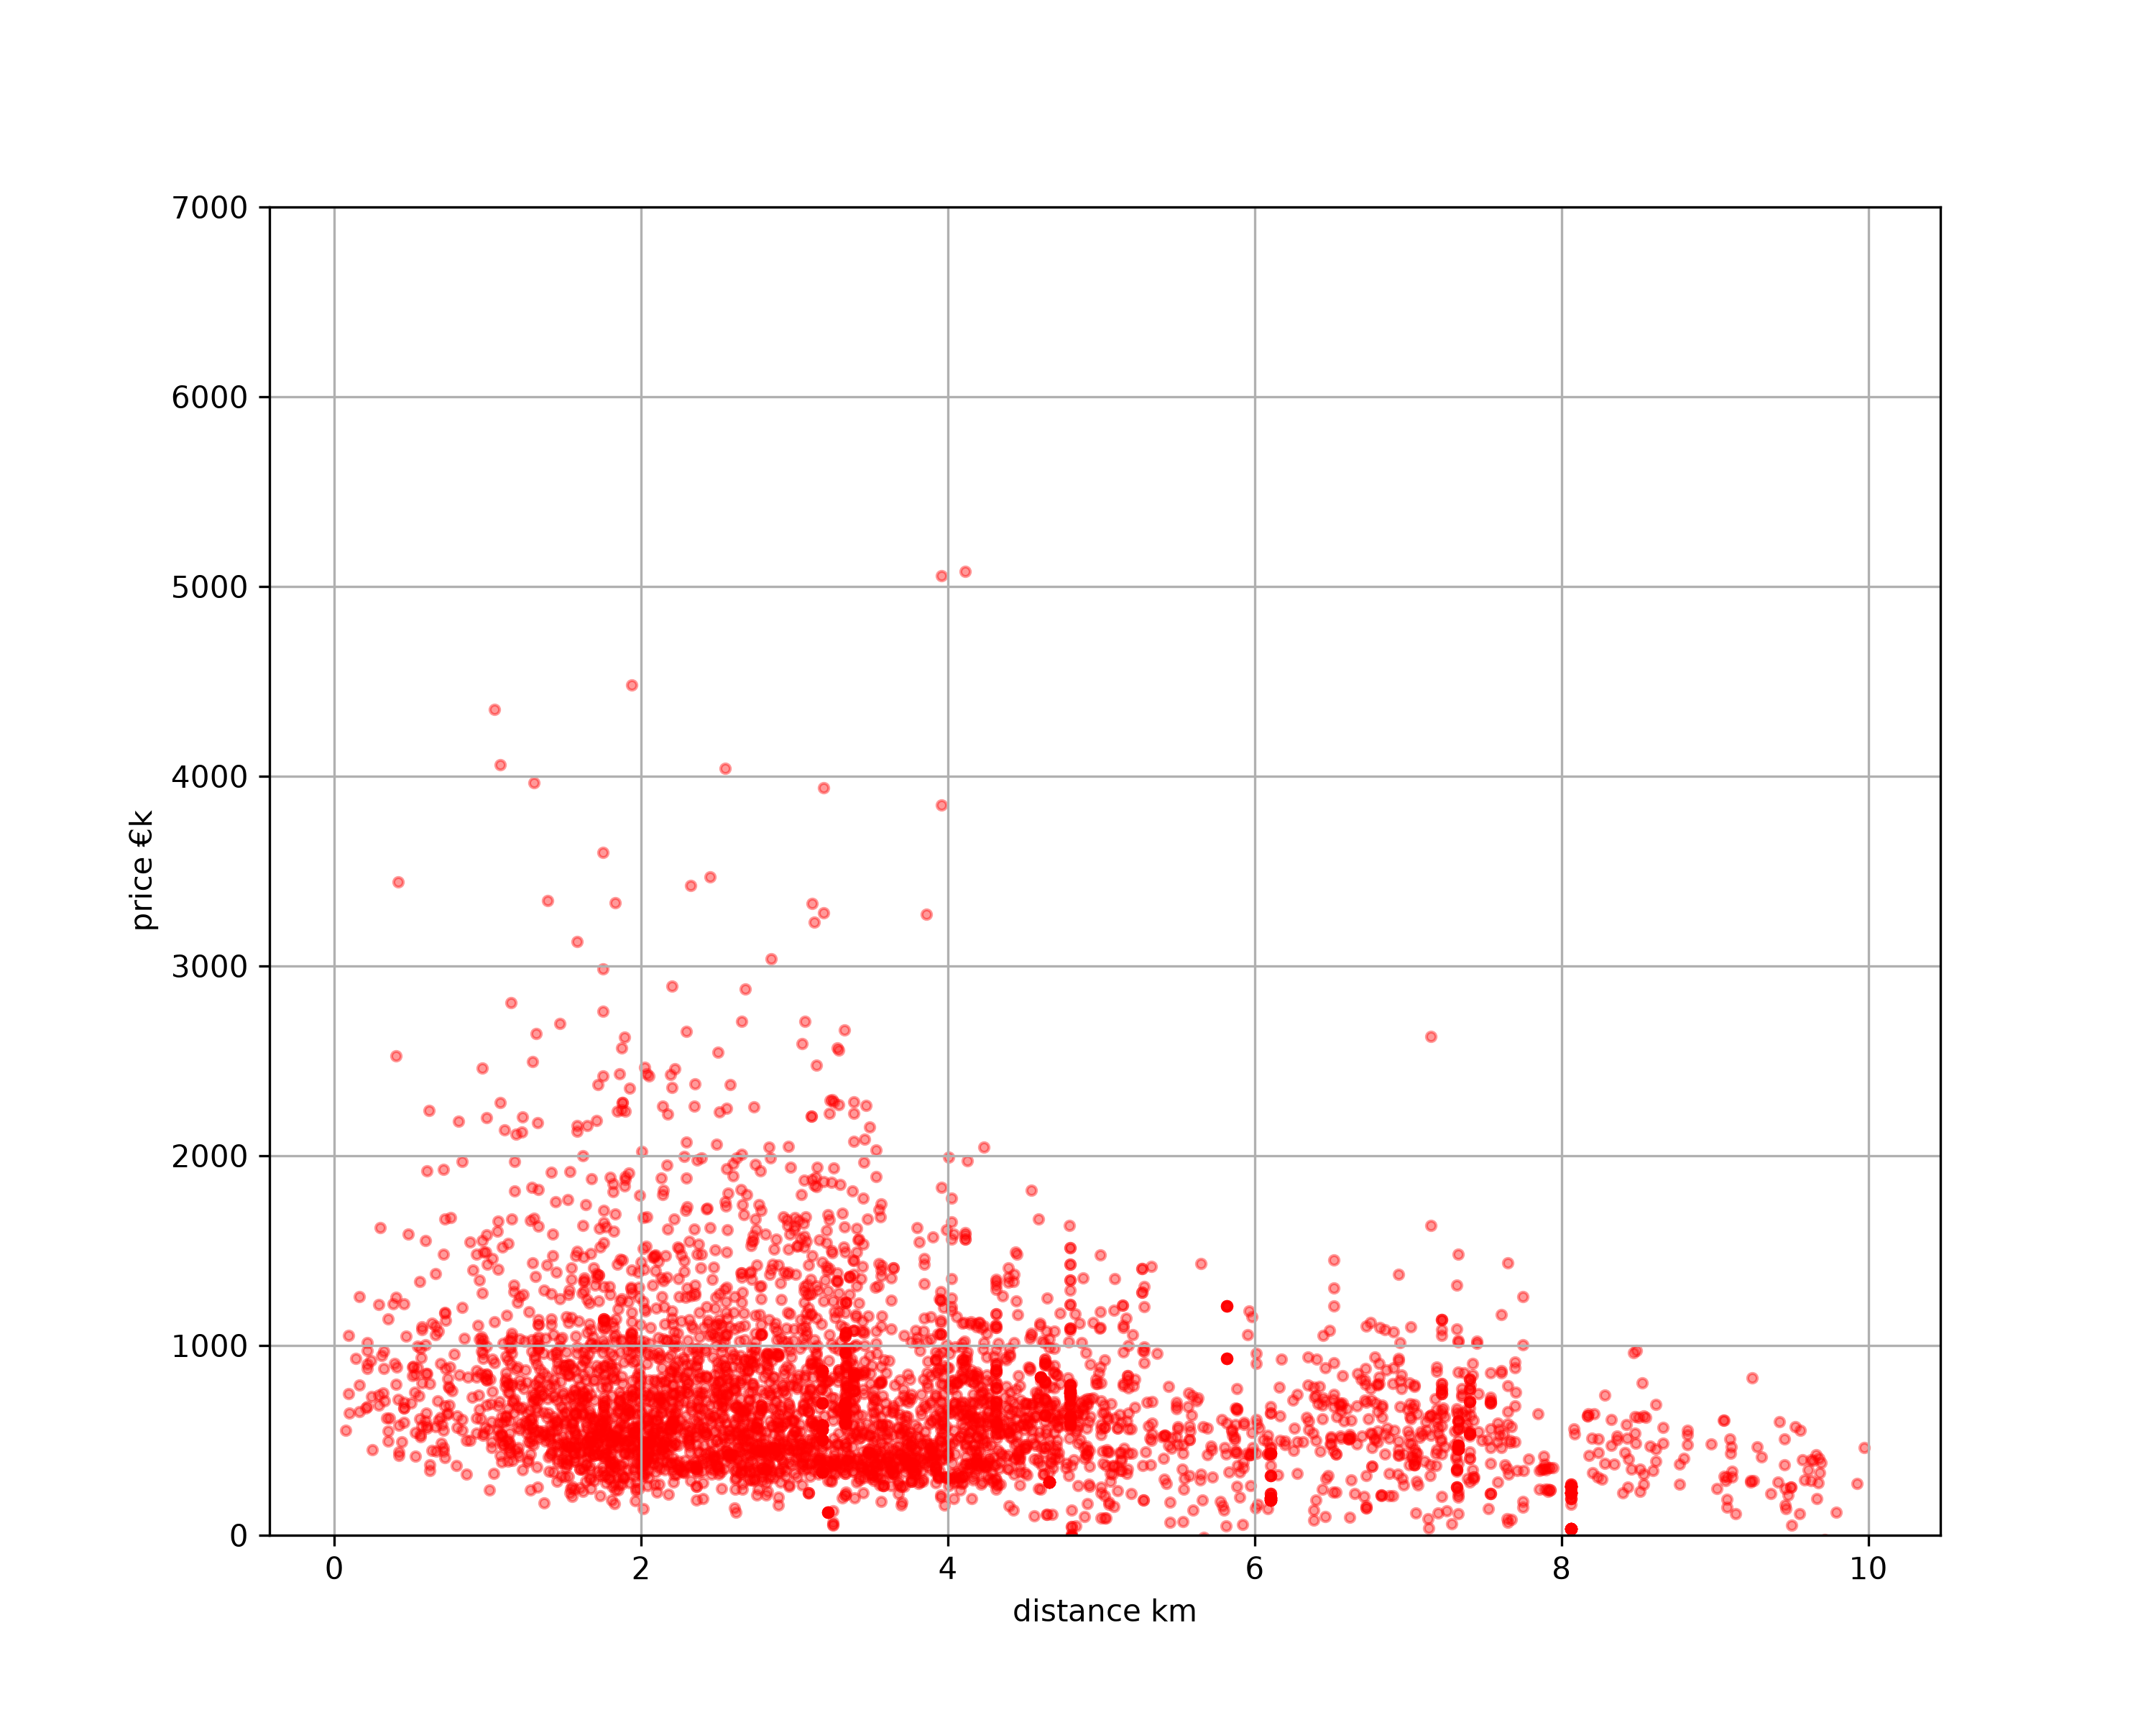
\includegraphics[width=0.9\textwidth]{graph_distance_nn.png}
    \caption{Distance against Price Predictions}
\end{figure}

The model was able to even capture the two spikes in price at distance 0 - 4km and 6 - 8km.


\begin{table}[H]
\centering
\begin{tabular}{|c|c|c|c|}
\hline
\# of inputs & average loss & $\mathrm{MAE}$ & $\mathrm{MAPE}$ \\
\hline
1 & $3.7487 {\times} 10^{-4}$ & 162.0 & 25.5\% \\
\hline
2 & $3.4844 {\times} 10^{-4}$ & 149.5 & 22.9\% \\
\hline
3 & $3.0009 {\times} 10^{-4}$ & 130.2 & 18.3\% \\
\hline
\end{tabular}
\end{table}


\end{document}